%%%%%%%%%%%%%%%%%%%%%%%%%%%%%%%%%%%%%%%%%
% University Assignment Title Page 
% LaTeX Template
% Version 1.0 (27/12/12)
%
% This template has been downloaded from:
% http://www.LaTeXTemplates.com
%
% Original author:
% WikiBooks (http://en.wikibooks.org/wiki/LaTeX/Title_Creation)
%
% License:
% CC BY-NC-SA 3.0 (http://creativecommons.org/licenses/by-nc-sa/3.0/)
% 
% Instructions for using this template:
% This title page is capable of being compiled as is. This is not useful for 
% including it in another document. To do this, you have two options: 
%
% 1) Copy/paste everything between \begin{document} and \end{document} 
% starting at \begin{titlepage} and paste this into another LaTeX file where you 
% want your title page.
% OR
% 2) Remove everything outside the \begin{titlepage} and \end{titlepage} and 
% move this file to the same directory as the LaTeX file you wish to add it to. 
% Then add \input{./title_page_1.tex} to your LaTeX file where you want your
% title page.
%
%%%%%%%%%%%%%%%%%%%%%%%%%%%%%%%%%%%%%%%%%
%\title{Title page with logo}
%----------------------------------------------------------------------------------------
%	PACKAGES AND OTHER DOCUMENT CONFIGURATIONS
%----------------------------------------------------------------------------------------

\documentclass[12pt]{article}
\usepackage[lithuanian]{babel}
\usepackage[L7x,T1]{fontenc}
\usepackage[utf8x]{inputenc}
\usepackage{amsmath}
\usepackage{graphicx}
\usepackage[colorinlistoftodos]{todonotes}
\usepackage{titlesec}
\usepackage{indentfirst}
\usepackage{float}
\usepackage{subcaption}
\usepackage{longtable}
\titlelabel{\thetitle.\quad}
\usepackage{tocloft}
\renewcommand{\cftsecleader}{\cftdotfill{\cftdotsep}}
\setlength{\parindent}{1cm} 

\usepackage{geometry}
 \geometry{
 a4paper,
 total={170mm,257mm},
 left=30mm,
 top=20mm,
 right=15mm,
 bottom=20mm,
 }

\usepackage{array}
\newcolumntype{L}[1]{>{\raggedright\let\newline\\\arraybackslash\hspace{0pt}}m{#1}}
\newcolumntype{C}[1]{>{\centering\let\newline\\\arraybackslash\hspace{0pt}}m{#1}}
\newcolumntype{R}[1]{>{\raggedleft\let\newline\\\arraybackslash\hspace{0pt}}m{#1}}

\begin{document}

\begin{titlepage}

\newcommand{\HRule}{\rule{\linewidth}{0.5mm}} % Defines a new command for the horizontal lines, change thickness here

\center % Center everything on the page
 
%----------------------------------------------------------------------------------------
%	HEADING SECTIONS
%----------------------------------------------------------------------------------------

\textsc{\LARGE BPN LT}\\[1.5cm] % Name of your university/college
\textsc{\Large IT skyrius}\\[0.5cm] % Major heading such as course name
\textsc{\large versija 1.0}\\[0.5cm] % Minor heading such as course title

%----------------------------------------------------------------------------------------
%	TITLE SECTION
%----------------------------------------------------------------------------------------

\HRule \\[0.4cm]
{ \huge \bfseries Skaitmeninės reklamos planavimo optimizavimo projektas.}\\[0.4cm] % Title of your document
\HRule \\[1.5cm]
 
%----------------------------------------------------------------------------------------
%	AUTHOR SECTION
%----------------------------------------------------------------------------------------

\begin{minipage}{0.4\textwidth}
\begin{flushleft} \large
\emph{Autorius:}\\
Gediminas Krasauskas % Your name
\end{flushleft}
\end{minipage}
~
\begin{minipage}{0.4\textwidth}
\begin{flushright} \large
\emph{Vadovas:} \\
Gedas Kučinskas % Supervisor's Name
\end{flushright}
\end{minipage}\\[2cm]

% If you don't want a supervisor, uncomment the two lines below and remove the section above
%\Large \emph{Author:}\\
%John \textsc{Smith}\\[3cm] % Your name

%----------------------------------------------------------------------------------------
%	DATE SECTION
%----------------------------------------------------------------------------------------

{\large \today}\\[2cm] % Date, change the \today to a set date if you want to be precise

%----------------------------------------------------------------------------------------
%	LOGO SECTION
%----------------------------------------------------------------------------------------


\includegraphics{Images/logo.png}\\[1cm] % Include a department/university logo - this will require the graphicx package
 
%----------------------------------------------------------------------------------------

\vfill % Fill the rest of the page with whitespace

\end{titlepage}


\begin{abstract}
Šis dokumentas yra skirtas įmonės UAB BPN LT kampanijos kūrimo optimizavimo bei automatizavimo projekto dokumentacijos aprašymui. Projektas buvo inicijuotas trišaliu sutarimu tarp: Vilniaus universiteto, į praktiką priimto studento Gedimino Krasausko ir įmonės BPN LT. Projektas buvo vystomas nuo 2019-02-04 iki 2019-04-12.
\end{abstract}


\pagebreak
\tableofcontents


\pagebreak
\section{Įvadas}

Dokumentacija sukurta siekiant dokumentuoti projekto vykdymo eigoje pasiektus rezultatus. Dokumentas turėtų būti naudingas įmonės BPN LT darbuotojams, kurie palaikys sukurtą projektą, taip pat potencialiai naujai į įmonę priimtiems praktikantams, kurie pratęs bei tobulins pradėtą projektą ar net kurs naują šio projekto pagrindu.

Naudojant dokumentaciją kaip šaltinį, skaitytojui turėtų tapti aišku ką galima nuveikti su programa, kokia yra projekto struktūra, kaip viekia programinis kodas ir ko iš jo tikėtis. Taip pat projekto tikslai, jam keliami reikalavimai bei užsakovų poreikiai.

Dokumentacija struktūrizuota į 7 skyrius. Antrame skyriuje aprašoma bendra projekto informacija. Trečiame nurodomos visos su projektu susijusios šalys ir asmenys bei jų kontaktai. Ketvirtame skyriuje aprašomi analizės rezultatai, t.y. projekto reikalavimų specifikacija. Penktas skyrius aprašo vartotojo dokumentaciją - tai kaip naudotis įrankiu nekreipiant dėmesio į kodo detales, kad būtų pasiektas norimas funkcionalumas.
Šeštame skyriuje nurodoma pagrindinė projekto dokumentacija: užduočių, klasių ir sekų diagramos, taip pat programinio kodo detali dokumentacija. Paskutinė dalis skirta autoriaus pastebėjimams bei rekomendacijoms ateičiai.



\pagebreak
\section{Projekto bendra informacija}
Su projektu susijusi bendra informacija pateikta 1 lentelėje.

\begin{table}[htb]
\centering
\caption{Bendra informacija}
\begin{tabular}{|L{6cm}|L{9.5cm}|}
\hline

Projekto pavadinimas & 
Skaitmeninės reklamos planavimo optimizacijos projektas     
\\ \hline

Projekto periodas & 
2019.02.04 - 2019.04.12     
\\ \hline

Projekte naudojamos technologijos & 
Google docs, Google Apps Script, JavaScript, HTML    
\\ \hline

Projekto užsakovas & 
UAB BPN LT        
\\ \hline

Projekto vadovas & 
Gedas Kučinskas        
\\ \hline

Projekto vystytojas & 
Gediminas Krasauskas        
\\ \hline

Projekto dokumentacijos direktorija & 
https://www.overleaf.com/2471937264qdvqdbngcnvv    
\\ \hline

Projekto dokumentacijos LaTeX direktorija & 
https://www.overleaf.com/2471937264qdvqdbngcnvv    
\\ \hline

Programinio kodo direktorija & 
https://www.overleaf.com/2471937264qdvqdbngcnvv    
\\ \hline


\end{tabular}
\end{table}


\pagebreak
\section{Suinteresuotos šalys}

Toliau pateikiama lentelė su visais, dalyvavusiais arba su projektu susijusiais asmenimis.

\begin{table}[htb]
\centering
\caption{Suinteresuotos šalys}
\begin{tabular}{|L{5.5cm}|L{4.5cm}|L{5cm}|}
\hline
\multicolumn{1}{|c|}{\textbf{Rolė/pareigos}} & 
\multicolumn{1}{c|}{\textbf{Asmuo}} & 
\multicolumn{1}{c|}{\textbf{Kontaktai}} \\ \hline

Praktikantas, projekto autorius &
Gediminas Krasauskas & 
gediminask.bpnlt.com, gedgeds@gmail.com, +37063490854 \\ \hline

Praktikos vadovas iš universiteto pusės & 
Romas Baronas & 
romas.baronas@mif.vu.lt \\ \hline

Praktikos vadovas iš įmonės pusės &
Gedas Kučinskas &
gedas@bpnlt.com, +37067246854 \\ \hline

Neoficialus praktikos vadovas dalykinės srities klausimais &
Kasparas Januitis &
kasparasj@bpnlt.com, +37060507282 \\ \hline
 
Neoficialus praktikos vadovas IT klausimais &
Deividas Balyševas &
deividasb@bpnlt.com, +37060914872 \\ \hline
 
Duomenų bazės kūrėjas &
Edvinas Pečiauskas &
edvinasp@bpnlt.com \\ \hline


\end{tabular}
\end{table}





%----------------------------------------------------------------------------------------
%	R E I K A L A V I M Ų      S P E C I F I K A C I J A
%----------------------------------------------------------------------------------------


\pagebreak
\section{Reikalavimų specifikacija}
Reikalavimų specifikacija buvo kuriama projekto vykdymo metu ją nuosekliai pildant pagal projektui keliamus reikalavimus. 


\subsection{Funkciniai reikalavimai}
Funkcinių reikalavimų stulpelių reikšmės:
\begin{itemize}
    \itemsep0em 
    \item ID - unikalus reikalavimo identifikatorius;
    \item Aprašymas - reikalavimo detalus aprašas.
\end{itemize}

{\centering

\begin{longtable}{|L{2cm}|L{13.5cm}|}
\caption{Funkcinių reikalavimų specifikacija}
\hline
\multicolumn{1}{|c|}{\textbf{ID}} & 
\multicolumn{1}{c|}{\textbf{Aprašymas}} \\ \hline

FR.0101 &
Sistema turi generuoti Media plano šabloną.
\\ \hline

FR.0102 &
Media plano šablonas generuojamas iš atidarytos skaičiuoklės bet kurio lapo.
\\ \hline

FR.0103 &
Vartotojas gali pasirinkti Media plano šablono kūrimą lietuvių arba anglų kalba.
\\ \hline

FR.0104 &
Naujai sukurto Media plano šablono skaičiuoklės lapo pavadinimas turi būti „Media planas“.
\\ \hline
  
FR.0105 &
Sukūrus Media planą vartotojas turi atsidurti naujai sukurtame skaičiuoklės lape.
\\ \hline
 
FR.0106 &
Kiekviename Media plano šablone turi būti pavaizduotas BPN LT logotipas, Meta duomenų antraščių ir reikšmių laukai bei pagrindinių stulpelių antraštės.
\\ \hline
 
FR.0107 &
Kiekviename Media plane esančius Meta duomenų laukus sudaro antraščių pavadinimai vertikaliose koordinatėse A1:A8 atitinkamai: \textit{Užsakovas}, \textit{Klientas}, \textit{Produktas}, \textit{Kampanija}, \textit{Periodas}, \textit{Šalis}, \textit{Kampanijos ID}, \textit{Kampanijos pavadinimas} arba angliški jų atitikmenys.
\\ \hline
  
FR.0108 &
Media plane esančio logotipo kairioji viršutinė viršūnė turi prasidėti C1 langelyje.
\\ \hline
  
FR.0109 &
Media plane esantys Meta duomenų reikšmių visi laukai turi būti tušti ir juos rankiniu būdu turi įvesti vartotojas.
\\ \hline
  
FR.0110 &
Media plano Meta duomenų reikšmių Periodo lauke, esančiame B5 langelyje, vartotojas turi įvesti datą formatu: YYYY.MM.DD-YYYY.MM.DD.
\\ \hline
  
FR.0111 &
Kiekviename Media plane esančius pagrindinių stulpelių laukus sudaro antraščių pavadinimai horizontaliose koordinatėse A10:P12 atitinkamai: \textit{Tiekėjas}, \textit{Tinklapis}, \textit{Aplinka}, \textit{Nukreipimas}, \textit{Ribojimas}, \textit{Skydelis, px}, \textit{Skydelio tipas}, \textit{Vienetas}, \textit{Kiekis}, \textit{Pirkimo tipas}, \textit{Viso}, \textit{Vieneto gross kaina}, \textit{Vieneto Neto kaina}, \textit{Gross kaina (EUR)}, \textit{Nuolaida (\%)}, \textit{Neto kaina (EUR)}  arba angliški jų atitikmenys.
\\ \hline
  
FR.0112 &
Kiekviename Media plane esančius papildomų stulpelių laukus sudaro antraščių pavadinimai horizontaliose koordinatėse Q10:S10 atitinkamai: \textit{Prognozės} ir antraščių pavadinimai horizontaliose koordinatėse Q11:S12 atitinkamai: \textit{Parodymai}, \textit{CTR}, \textit{Nukreipimai} arba angliški jų atitikmenys.
\\ \hline  
  
FR.0113 &
Media plane turi būti meniu pasirinkimas automatiškai generuoti įrašus.
\\ \hline  
  
FR.0114 &
Media plane turi būti meniu pasirinkimas automatiškai generuoti kalendorių.
\\ \hline  
  
FR.0115 &
Media plane turi būti meniu pasirinkimas automatiškai generuoti užsakymą.
\\ \hline  
  
FR.0116 &
Media plane turi būti meniu pasirinkimas automatiškai generuoti parašą.
\\ \hline  

FR.0117 &
Media plane turi būti pasirinkimas automatiškai atnaujinti duomenų bazę.
\\ \hline  
  
FR.0201 &
Vartotojas, pasirinkęs automatinį įrašų generavimą, turi galimybę įvesti įrašų skaičių.
\\ \hline  

FR.0202 &
Įvestas įrašų skaičius atvaizduojamas koordinatėse A14:SN, kur N - vartotojo įvestas įrašų skaičius + 13.
\\ \hline  
  
FR.0203 &
Vartotojui iš naujo pasirinkus automatinį įrašų generavimą ankstesni įrašai negali būti ištrinami.
\\ \hline  

FR.0204 &
Sistemai sugeneravus įrašus vartotojas stulpelyje A iš pasirenkamojo sąrašo turi galimybę pasirinkti norimą tiekėją.
\\ \hline  
  
FR.0205 &
Pasirenkamieji sąrašai Media plane yra stulpeliuose, pavadinimais: \textit{Tiekėjas}, \textit{Tinklapis}, \textit{Aplinka}, \textit{Nukreipimas}, \textit{Skydelis, px}, \textit{Skydelio tipas}.
\\ \hline 
  
FR.0206 &
Pasirinkus reikšmę stulpelyje \textit{Tiekėjas}, turi atsirasti naujas pasirenkamasis sąrašas stulpelyje \textit{Tinklapis}, ir t.t.
\\ \hline  

FR.0207 &
Jeigu pasirenkamajame sąraše yra tik viena reikšmė, ji stulpelyje atsiranda automatiškai.
\\ \hline  
  
FR.0208 &
Vartotojas visada gali pakeisti pasirenkamojo sąrašo reikšmes.
\\ \hline  
  
FR.0209 &
Vartotojas rankiniu būdu įveda atitinkamų stulpelių įrašų reikšmes: \textit{Ribojimas}, \textit{Vienetas}, \textit{Pirkimo tipas}, \textit{Vieneto gross kaina}, \textit{Nuolaida (\%)}, \textit{CTR}.
\\ \hline  
  
FR.0210 &
stulpelių įrašų reikšmės: \textit{Vieneto gross kaina}, \textit{Nuolaida (\%)}, \textit{CTR} yra skaitinės reikšmės ir atitinka formatą: X,YY.
\\ \hline  

FR.0211 &
stulpelių įrašų reikšmės: \textit{Kiekis}, \textit{Viso}, \textit{Vieneto neto kaina}, \textit{Gross kaina (EUR)}, \textit{Neto kaina (EUR)}, \textit{Parodymai}, \textit{Nukreipimai} yra priklausomos nuo kitų stulpelių reikšmių ir užpildomos automatiškai pagal formules.
\\ \hline  
  
FR.0212 &
stulpelio \textit{Kiekis} įrašų reikšmės užpildomos pagal formulę: visų kalendoriuje esančių reikšmių sumą.
\\ \hline    
  
FR.0213 &
stulpelio \textit{Viso} įrašų reikšmės užpildomos pagal formulę: \textit{Vienetas} * \textit{Kiekis}.
\\ \hline  
  
FR.0214 &
stulpelio \textit{Vieneto neto kaina} įrašų reikšmės užpildomos pagal formulę: teigiama \textit{Vieneto gross kaina} - \textit{Vieneto gross kaina} * \textit{Nuolaida}.
\\ \hline    
  
FR.0215 &
stulpelio \textit{Gross kaina (EUR)} įrašų reikšmės užpildomos pagal formulę: \textit{Vieneto gross kaina} * \textit{Kiekis}.
\\ \hline    
  
FR.0216 &
stulpelio \textit{Neto kaina (EUR)} įrašų reikšmės užpildomos pagal formulę: \textit{Vieneto neto kaina} * \textit{Kiekis}.
\\ \hline  
  
FR.0217 &
stulpelio \textit{Parodymai} įrašų reikšmės užpildomos pagal formulę: \textit{Vienetas} * \textit{Kiekis}.
\\ \hline    
  
FR.0218 &
stulpelio \textit{Nukreipimai} įrašų reikšmės užpildomos pagal formulę: \textit{Parodymai} * \textit{CTR}.
\\ \hline    
  
FR.0301 &
Vartotojui pasirinkus automatinį kalendoriaus generavimą, sugeneruojamas kalendorius laukuose T10:X13 pagal Meta duomenų Periodo reikšmę.
\\ \hline    
  
FR.0302 &
Sugeneruotas kalendorius turi rodyti mėnesį laukuose T10:X10, savaitės numerį laukuose T11:X11, savaitės dieną laukuose T12:X12 ir mėnesio dienos numerį laukuose T13:X13.
\\ \hline  
  
FR.0303 &
Sugeneruoto kalendoriaus periodas turi prasidėti 3 dienomis ansčiau nurodyto periodo ir 3 dienomis vėliau nurodyto periodo.
\\ \hline  
    
FR.0401 &
Vartotojui pasirinkus automatinį parašo generavimą, sugeneruojami parašo laukai 5 eilutėmis žemiau paskutinės netuščios eilutės skaičiuoklės lape.
\\ \hline    
    
FR.0402 &
Sugeneruotas parašas turi turėti tokias laukų antraštes: \textit{Vėliausias patvirtinimas iki}, \textit{Kliento patvirtinimas}, \textit{Vardas, pavardė}, \textit{Data}, \textit{Parašas}.
\\ \hline    
    
FR.0403 &
Sugeneruotame paraše turi būti sukurtas laukas su vėliausio patvirtinimo data, sutampančia su Meta duomenų Periodo reikšmės pradžia - 1 diena.
\\ \hline    
    
FR.0501 &
Sugeneruota arba atnaujinta duomenų bazė turi nesimatyti vartotojui.
\\ \hline    
    
FR.0601 &
Užsakymo šablonas generuojamas iš atidarytos skaičiuoklės Media plano lapo.
\\ \hline    
  
FR.0602 &
Vartotojas privalo pasirinkti Užsakymo šablono kūrimą lietuvių arba anglų kalba.
\\ \hline    
  
FR.0603 &
Vartotojas privalo pasirinkti kanalą Užsakymo šablono kūrimui.
\\ \hline    
  
FR.0604 &
Naujai sukurto Užsakymo šablono skaičiuoklės lapo pavadinimas turi būti \textit{Order} \textit{Pasirinktas kanalas}.
\\ \hline    
  
FR.0605 &
Sukūrus Užsakymą vartotojas turi atsidurti naujai sukurtame skaičiuoklės lape.
\\ \hline    
  
FR.0606 &
Visos su konkrečiu užsakymu susijusios reikšmės turi būti nukopijuotos į užsakymą tuo pačiu išdėstymu, tačiau be papildomų Prognozių stulpelių ir Meta duomenų: \textit{Kampanijos ID} bei \textit{Kampanijos pavadinimas}.
\\ \hline    
  
FR.0607 &
Užsakyme turi būti apskaičiuojami rodikliai, pateikiami po įrašais: \textit{Gross kaina}, \textit{Nuolaida} ir \textit{Neto kaina}.
\\ \hline   
  
\end{longtable}

}

\subsection{Nefunkciniai reikalavimai}

Nefunkcinių reikalavimų stulpelių reikšmės:
\begin{itemize}
    \itemsep0em 
    \item ID - unikalus reikalavimo identifikatorius;
    \item Aprašymas - reikalavimo detalus aprašas.
\end{itemize}

{\centering

\begin{longtable}{|L{2cm}|L{13cm}|}
\caption{Nefunkcinių reikalavimų specifikacija}
\hline
\multicolumn{1}{|c|}{\textbf{ID}} & 
\multicolumn{1}{c|}{\textbf{Aprašymas}}  \\ \hline

NFR.0001 &
Sistema turi pritaikoma naudojimui Google Sheets aplikacijoje. 
\\ \hline
  
NFR.0002 &
Sistema turi būti parašyta Google Apps Script programavimo kalba.
\\ \hline
  
NFR.0003 &
Sistema turi būti prieinama visiems BPN LT domeno naudotojams ir neprieinama visiems, esantiems už šio domeno ribų.
\\ \hline

NFR.0004 &
Sistema turi naudoti duomenų bazės įrašus, patalpintus atskiroje skaičiuoklėje.
\\ \hline
  
NFR.0005 &
Išorinės duomenų bazės nė vienas laukas negali būti tuščias.
\\ \hline
  
NFR.0006 &
Sistema gali naudotis iki 20 žmonių vienu metu.
\\ \hline
  
NFR.0007 &
Bet koks veiksmas sistemai atlikti netrunka ilgiau nei 5 sekundes.
\\ \hline
  
\end{longtable}

}
  
\subsection{Kosmetiniai reikalavimai}

Kosmetinių reikalavimų stulpelių reikšmės:
\begin{itemize}
    \itemsep0em 
    \item ID - unikalus reikalavimo identifikatorius;
    \item Aprašymas - reikalavimo detalus aprašas.
\end{itemize}

{\centering

\begin{longtable}{|L{1.8cm}|L{14cm}|}
\caption{Kosmetinių reikalavimų specifikacija}
\hline
\multicolumn{1}{|c|}{\textbf{ID}} & 
\multicolumn{1}{c|}{\textbf{Aprašymas}} \\ \hline

KR.0101 &
Media plano ir Užsakymo šablonų globalūs šriftai turi būti „Tahoma“.
\\ \hline
  
KR.0102 &
Media plano ir Užsakymo šablonuose turi būti pašalintas tinklelis.
\\ \hline
  
KR.0103 &
Media plano ir Užsakymo Meta duomenų antraščių ir rezultatų, visų stulpelių antraščių, Media plano parašo ir kalendoriaus antraščių fono spalvos turi būti pilkos.
\\ \hline
  
KR.0104 &
Media plano ir Užsakymo kalendoriaus antraščių šeštadienio ir sekmadienio savaitės dienų pavadinimų fono spalvos turi būti tamsiai pilkos.
\\ \hline
  
KR.0105 &
Media plano ir Užsakymo Meta duomenų antraščių ir rezultatų laukų sienelės turi būti užpildytos tiesiu būdu iš visų pusių tiek išorėje, tiek viduje.
\\ \hline  
  
KR.0106 &
Media plano ir Užsakymo pagrindinių stulpelių antraščių sienelės turi būti užpildytos tiesiu būdu iš visų pusių tiek išorėje, tiek viduje.
\\ \hline  
  
KR.0107 &
Media plano ir Užsakymo kalendoriaus antraščių sienelės turi būti užpildytos tiesiu būdu iš visų pusių tiek išorėje, tiek viduje.
\\ \hline  
  
KR.0108 &
Media plano ir Užsakymo įrašų duomenų laukų sienelės turi būti užpildytos tiesiu būdu iš visų pusių tiek išorėje, tiek viduje.
\\ \hline  
  
KR.0109 &
Media plano ir Užsakymo kalendoriaus įrašų laukų sienelės turi būti užpildytos taškeliniu būdu iš visų pusių tiek išorėje, tiek viduje.
\\ \hline  

KR.0110 &
Media plano ir Užsakymo Meta duomenų antraščių ir rezultatų laukų šrifto dydis turi būti 8, visų kitų laukų 10.
\\ \hline

KR.0111 &
Užsakymo šablone pirmieji 2 stulpeliai iš kairės turi būti stacionarioje pozicijoje ir slenkant per lapą nejudėti.
\\ \hline
  
\end{longtable}

}



%----------------------------------------------------------------------------------------
%	V A R T O T O J O      D O K U M E N T A C I J A
%----------------------------------------------------------------------------------------


\pagebreak
\section{Vartotojo dokumentacija}
Ši dokumentacijos dalis skirta asmenims (labiausiai tikėtina - projektų vadovams), kurie naudosis suskurta sistema. Vartotojo dokumentacija turėtų pasitarnauti kaip instrukcijų rinkinys ir mokomoji medžiaga. Vartotojo dokumentacija suskirstyta į skirtingas dalis pagal vykdomas užduotis, prie kiekvienos pateikiant grafinę informaciją, instrukcijas rekomendacijas bei galimas problemas.

\subsection{Programinio kodo veikimo patikra}
Atidarius skaičiuoklės dokumentą (angl. \textit{Spreadsheet}) ir jam užsikrovus, sužinoti ar skaičiuoklėje yra įgalintas Google Apps Script failas, galime tik atlikę pažingsninę patikrą. Naudotojas turėtų išvysti atsiradusius 2 naujus meniu pasirinkimus: „Šablonai“ ir „Parankiniai“ (žr. 1 pav.). Meniu pasirinkimas „Šablonai“ turėtų atverti sub-meniu iš 2 elementų: „Media plano šablonas“ ir „Užsakymo šablonas“(žr. 2 pav.). Meniu pasirinkimas „Parankiniai“ turėtų atverti sub-meniu iš 4 elementų: „Atnaujinti duomenų bazę“, „Generuoti įrašus“, „Generuoti kalendorių“ ir „Užbaigti šabloną“(žr. 3 pav.).

\begin{figure}[H]
    \centering
    
\includegraphics[scale=0.9]{Images/Screenshots/menu-options.PNG}
    \caption{Nauji meniu pasirinkimai}
    \label{img:model}
\end{figure}

\begin{figure}[h]
    \centering
    \begin{minipage}{0.45\textwidth}
        \centering
        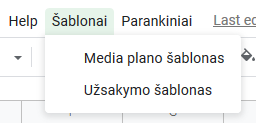
\includegraphics[scale=0.9]{Images/Screenshots/menu-template-options.PNG} 
        \caption{„Šablonai“ sub-meniu}
    \end{minipage}\hfill
    \begin{minipage}{0.45\textwidth}
        \centering
        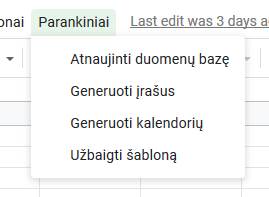
\includegraphics[scale=0.9]{Images/Screenshots/menu-other-options.PNG} 
        \caption{„Parankiniai“ sub-meniu}
    \end{minipage}
\end{figure}

\subsection{Media plano kūrimas}
Media plano kūrimas yra esminė ir pati pirmoji užduotis, kurią atlieka projekto vadovas. Neatlikus šios užduoties kitų užduočių taip pat negalima atlikinėti.

\bigskip
Media plano kūrimo instrukcijos: 
\begin{enumerate}
    \itemsep0em 
    \item Paspausti ant meniu pasirinkimo „Šablonai“ (žr. 1 pav.);
    \item Paspausti ant sub-meniu pasirinkimo „Media plano šablonas“ (žr. 2 pav.);
    \item Palaukti, kol atsidarys dialogo langas (modalas) (žr. 4 pav.);
    \item Pasirinkti norimą Media plano kalbą (žr. 4 pav.);
    \item Paspausti mygtuką „Kurti Media planą“ (žr. 4 pav.);
    \item Palaukti, kol bus įvykdytas programinis kodas, t.y. sukuriamas naujas skaičiuoklės lapas pavadinimu „Media planas“ su Media plano griaučiais (žr. 6 pav.): plano pagrindine informacija, BPN logotipu ir stulpelių pavadinimais. 
\end{enumerate}

\bigskip
Rekomendacijos:
\begin{itemize}
    \itemsep0em 
    \item Rekomenduotina, kad viename skaičiuoklės faile būtų tik vienas Media planas. Jeigu reikia 2 ar daugiau planų, patartina kurti naujus skaičiuoklių failus ir kiekviename atitinkamai vykdyti visus žingsnius nuo 1 punkto. Vis dėlto, jeigu būtina turėti 2 planus vienoje skaičiuoklėje, reikia pervadinti esamą Media plano lapo (angl. \textit{Sheet}) pavadinimą į naują (žr. punktas apačioje). Tačiau šitaip naudotojas prisiima riziką, kad programinis kodas veiks nekorektiškai;
    \item Jeigu Media plano lapą reikia pervadinti, yra būtina, kad naujajame pavadinime būtų nepertraukiamas ir tikslus žodžių junginys „Media planas“;
    \item 3 punktas. Norint išeiti iš dialogo lango, paspausti mygtuką „Uždaryti“ (žr. 4 pav.);
    \item 4 punktas. Numatytoji kalba - lietuvių (LT), tačiau galima pasirinkti ir anglų kalbą (EN) (žr. 4 pav.);
    \item 6 punktas. Kaskart sukuriant naują Media planą yra sukuriama lokali duomenų bazės kopija atskirame skaičiuoklės lape, tačiau projekto vadovui ji yra nematoma. Tam, kad projektų vadovas išvystų šią duomenų bazę, reikia ją pasirinkti (žr. 7 pav.). 
\end{itemize}

\bigskip
Galimos problemos:
\begin{itemize}
    \itemsep0em 
    \item 5 punktas. Paspaudus mygtuką „Kurti Media planą“ nieko nevyksta. Tokiu atveju reikia pakartoti viską iš naujo nuo 1 punkto, tik lėčiau spausti mygtukus;
    \item 5 punktas. Paspaudus mygtuką „Kurti Media planą“ atsidaro pranešimas (žr. 5 pav.). Tokiu atveju reikia paspausti „Ok“. Tai reiškia, kad esamoje skaičiuoklėje jau yra Media planas. Vienu metu gali būti tik 1 lapas tuo pačiu unikaliu pavadinimu;
    \item 6 punktas. Logotipas visada yra užkraunamas, tačiau ne visada matomas. Jeigu logotipas nesimato, reikia pereiti į bet kokį atidarytoje skaičiuoklėje esantį lapą ir grįžti atgal į sugeneruotą Media plano lapą.
\end{itemize}

\begin{figure}[h]
    \centering
    \begin{minipage}{0.45\textwidth}
        \centering
        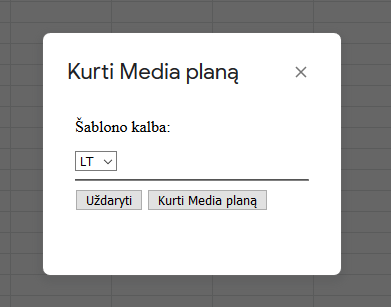
\includegraphics[scale=0.6]{Images/Screenshots/modal-media-plan.PNG} 
        \caption{Media plano kūrimo dialogas}
    \end{minipage}\hfill
    \begin{minipage}{0.45\textwidth}
        \centering
        
\includegraphics[scale=0.8]{Images/Screenshots/modal-media-plan-alert.PNG} 
        \caption{Media plano kūrimo klaidos pranešimas}
    \end{minipage}
\end{figure}

\begin{figure}[H]
    \centering
    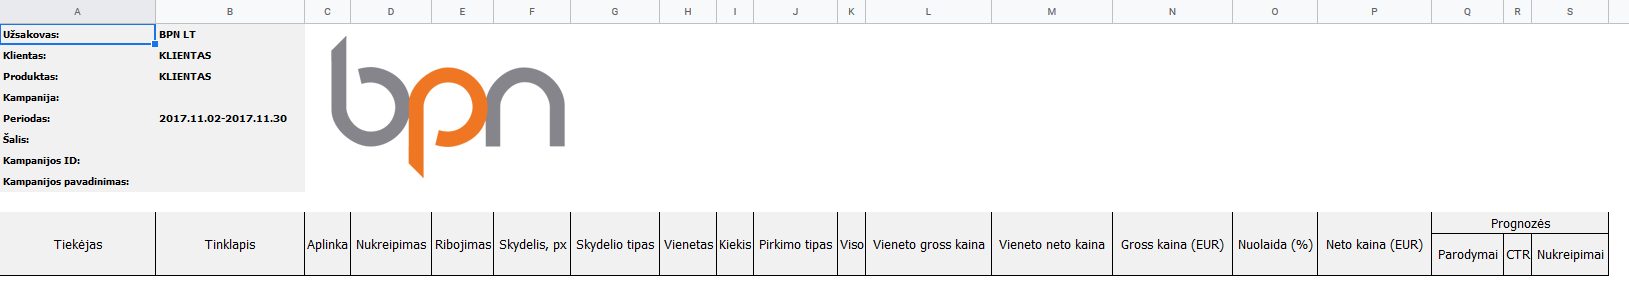
\includegraphics[scale=0.35]{Images/Screenshots/media-plan-generic.PNG}
    \caption{Media plano griaučiai}
    \label{img:model}
\end{figure}

\subsection{Duomenų bazės atnaujinimas}
Jau žinome, kad lokali duomenų bazė yra sukuriama kartu su Media plano šablonu. Tačiau yra tvejų, kada gali tekti pasirinkti duomenų bazės atnaujinimo užduotį:
\begin{itemize}
    \itemsep0em 
    \item Kuriant Media planą realiu laiku pasikeitė nuotolinės duomenų bazės reikšmės;
    \item Projektų vadovas netyčia ištrynė lokalią duomenų bazę.
\end{itemize}

\bigskip
Duomenų bazės atnaujinimo instrukcijos: 
\begin{enumerate}
    \itemsep0em 
    \item Nueiti į Media plano skaičiuoklės lapą;
    \item Paspausti ant meniu pasirinkimo „Parankiniai“ (žr. 1 pav.);
    \item Paspausti ant sub-meniu pasirinkimo „Atnaujinti duomenų bazę“ (žr. 3 pav.);
    \item Palaukti, kol bus įvykdytas programinis kodas. 
\end{enumerate}

\bigskip
Rekomendacijos:
\begin{itemize}
    \itemsep0em 
    \item Norint patikrinti ar atnaujinimas pavyko sėkmingai, reikia patikrinti ar duomenų bazė yra sukurta (žr. 7 pav.).
\end{itemize}

\bigskip
Galimos problemos:
\begin{itemize}
    \itemsep0em 
    \item 4 punktas. Paspaudus mygtuką „Atnaujinti duomenų bazę“ atsidaro pranešimas (žr. 8 pav.). Tokiu atveju reikia paspausti „Ok“. Tai reiškia, meniu pasirinkimas buvo pasirinktas ne iš Media plano skaičiuoklės lapo. Kad atnaujinimas pavyktų, reikia patikrinti ar tikrai esate media plane ir pakartoti viską nuo 1 punkto. 
\end{itemize}

\begin{figure}[h]
    \centering
    \begin{minipage}{0.45\textwidth}
        \centering
        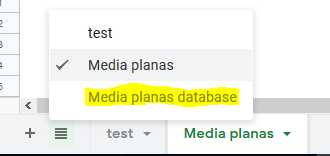
\includegraphics[scale=0.8]{Images/Screenshots/media-plan-hidden-database.PNG} 
        \caption{Paslėpta duomenų bazė}
    \end{minipage}\hfill
    \begin{minipage}{0.45\textwidth}
        \centering
        
\includegraphics[scale=0.6]{Images/Screenshots/media-plan-database-update-alert.PNG} 
        \caption{Duomenų Bazės atnaujinimo klaida}
    \end{minipage}
\end{figure}

\subsection{Įrašų generavimas}
Įrašų generavimas media plane yra viena svarbiausių pagalbinių funkcijų, be kurios nebūtų galima pildyti plano. Įrašų generavimą galima tlikti bet kada.

\bigskip
Įrašų generavimo instrukcijos: 
\begin{enumerate}
    \itemsep0em 
    \item Nueiti į Media plano skaičiuoklės lapą;
    \item Paspausti ant meniu pasirinkimo „Parankiniai“ (žr. 1 pav.);
    \item Paspausti ant sub-meniu pasirinkimo „Generuoti įrašus“ (žr. 3 pav.);
    \item Palaukti, kol atsidarys dialogo langas (modalas) (žr. 9 pav.);
    \item Įvesti norimą įrašų skaičių (žr. 9 pav.);
    \item Paspausti mygtuką „Ok“ (žr. 9 pav.);
    \item Palaukti, kol bus sugeneruoti įrašų laukai (žr. 10 pav.).
\end{enumerate}

\bigskip
Rekomendacijos:
\begin{itemize}
    \itemsep0em 
    \item 1 punktas. Įrašai gali būti generuojami tik media plano skaičiuoklės lape;
    \item Rekomenduotina iš anksto žinoti, kiek įrašų planui reikės, tačiau pritrūkus įrašų laukams, funkciją galima atlikti iš naujo;
    \item Įvedama skaitinė įrašų reikšmė visada yra absoliuti, t.y. jei prieš tai turėjome 10 įrašų ir mums reikia papildomų 4, 5 punkte reikės įvesti 14, t.y. 10 + 4;
    \item 5 punkte pasirinkus naują įrašų skaičių, esami įrašai skaičiuoklėje išsisaugo. Pavyzdžiui, turint 10 įrašų eilučių ir 5 punkte įvedus skaičių 8, paskutinės 2 įrašų eilutės nebus pašalintos, kaip ir pirmos 8, jeigu ten jau buvo įvestos reikšmės;
    \item Norint pašalinti įrašų eilutes, tą reikia atlikti renkiniu būdu;
    \item 5 punkte visada reikia vesti tik natūraliuosius sveikus skaičius.
\end{itemize}

\bigskip
Galimos problemos:
\begin{itemize}
    \itemsep0em 
    \item 3 punktas. Paspaudus mygtuką „Generuoti įrašus“ nieko nevyksta. Reikia patikrinti, ar tikrai esate Media plano skaičiuoklės lape. Pakartoti viską nuo 1 punkto.
\end{itemize}

\begin{figure}[H]
    \centering
    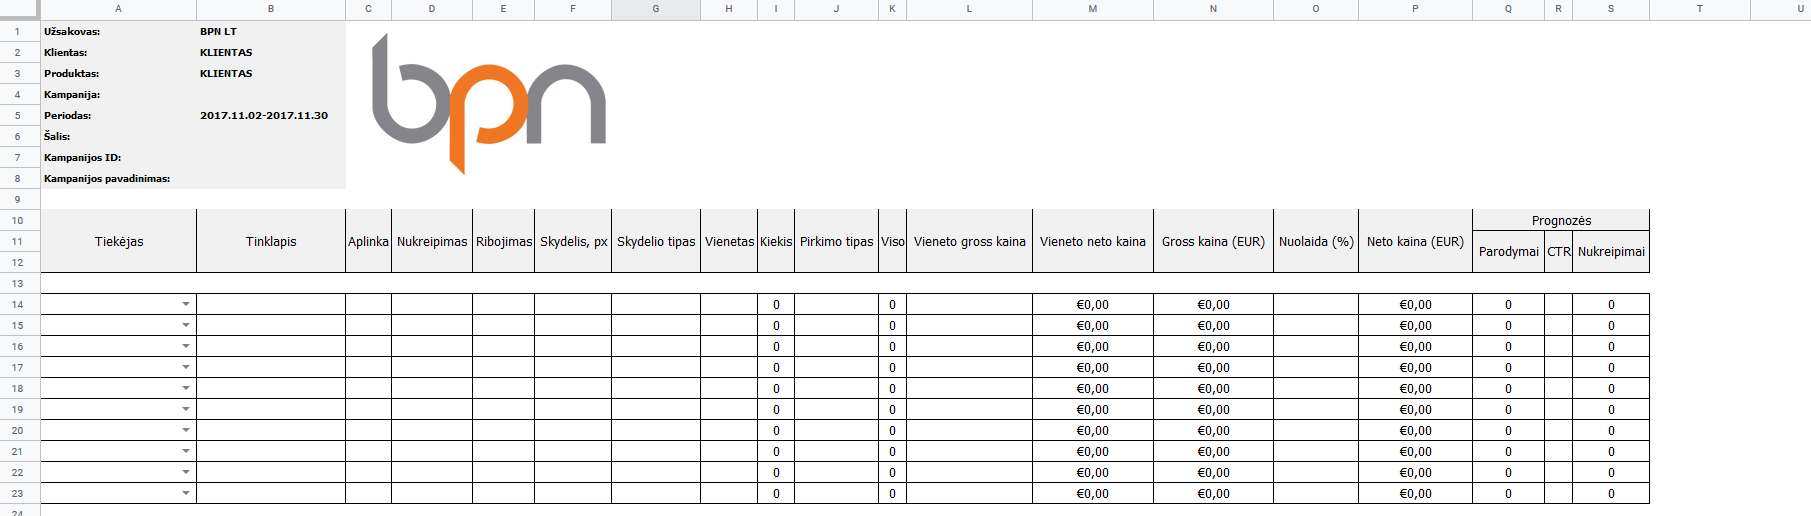
\includegraphics[scale=0.35]{Images/Screenshots/generated-records.PNG}
    \caption{Sugeneruoti įrašai}
    \label{img:model}
\end{figure}

\begin{figure}[h]
    \centering
    \begin{minipage}{0.45\textwidth}
        \centering
        
\includegraphics[scale=0.7]{Images/Screenshots/modal-generate-records.PNG} 
        \caption{Įrašų kūrimo dialogas}
    \end{minipage}\hfill
    \begin{minipage}{0.45\textwidth}
        \centering
        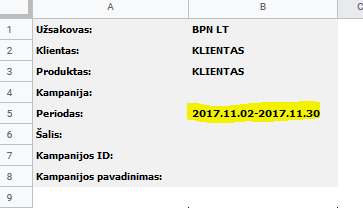
\includegraphics[scale=0.7]{Images/Screenshots/calendar-period-creation.PNG} 
        \caption{Periodo įvedimo laukas}
    \end{minipage}
\end{figure}

\subsection{Kalendoriaus generavimas}
Kalendoriaus generavimas media plane yra pagalbinė funkcija. Kalendoriaus generavimą galima atlikti bet kada - tiek prieš įrašų generavimą, tiek po jo.

\bigskip
Kalendoriaus generavimo instrukcijos: 
\begin{enumerate}
    \itemsep0em 
    \item Nueiti į Media plano skaičiuoklės lapą.
    \item Nueiti į skaičiuoklės B5 langelį ir įvesti norimą periodą (žr. 11 pav.).
    \item Paspausti ant meniu pasirinkimo „Parankiniai“ (žr. 1 pav.);
    \item Paspausti ant sub-meniu pasirinkimo „Generuoti kalendorių“ (žr. 3 pav.);
    \item Palaukti, kol programa įvykdys programinį kodą ir atsiras kalendorius (žr. 12 pav.);
\end{enumerate}

\bigskip
Rekomendacijos:
\begin{itemize}
    \itemsep0em 
    \item Kalendorius gali būti kuriamas tik iš Media plano skaičiuoklės lapo;
    \item Įvedamas periodas privalo būti B5 langelyje;
    \item Įvedamas periodas privalo būti atitinkamo formato: YYYY.MM.DD-YYYY.MM.DD; Pavyzdys - 2019.10.22-2019.12.31;
    \item Įvedamas periodas privalo būti korektiškas, t.y. periodo pradžia negali būti vėliau negu periodo pabaiga, datos turi būti realistiškos (pvz. 2019.02.55);
    \item Norint pakeisti kalendoriaus periodą, tereikia pakeisti B5 langelio reikšmę ir atlikti viską nuo 1 punkto. Kalendorius bus ištrintas ir sugeneruotas iš naujo. Visos kitos reikšmės kalendoriaus laukuose liks nepakeistos. Pasirinkus naują trumpesnį kalendoriaus periodą, kalendoriaus reikšmės, nepatenkančios į naują periodą liks neištrintos, kaip ir reikšmės, patenkančios į naują periodą. Šias reikšmes reikia ištrinti rankiniu būdu.
\end{itemize}

\bigskip
Galimos problemos:
\begin{itemize}
    \itemsep0em 
    \item 4 punktas. Paspaudus mygtuką „Generuoti kalendorių“ nieko nevyksta. Reikia patikrinti, ar tikrai esate Media plano skaičiuoklės lape. Pakartoti viską nuo 1 punkto;
    \item 4 punktas. Paspaudus mygtuką „Generuoti kalendorių“, atsidaro pranešimas (žr. 13 pav. Tokiu atveju reikia paspausti mygtuką „Ok“. Tai reiškia, kad įvesto periodo pradžia yra vėliau, negu įvesto periodo pabaiga;
    \item 4 punktas. Paspaudus mygtuką „Generuoti kalendorių“, atsidaro pranešimas (žr. 13 pav. Tai reiškia, kad įvestas periodas yra ilgesnis negu 100 dienų. Jeigu norima generuoti periodą, ilgesnį nei 100 dienų, reikia spausti mygtuką „Yes“. Priešingu atveju reikia spausti mygtuką „No“ ir pakeisti periodo reikšmę.
\end{itemize}

\begin{figure}[h]
    \centering
    \begin{minipage}{0.45\textwidth}
        \centering
        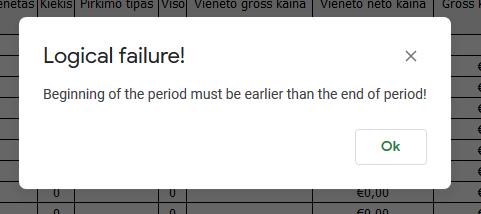
\includegraphics[scale=0.6]{Images/Screenshots/calendar-creation-logical-failure.PNG} 
        \caption{Periodo įvesties klaida}
    \end{minipage}\hfill
    \begin{minipage}{0.45\textwidth}
        \centering
        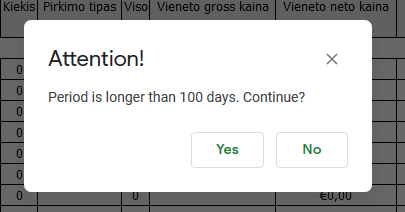
\includegraphics[scale=0.6]{Images/Screenshots/calendar-creation-long-period.PNG}
        \caption{Periodo įvesties perspėjimas}
    \end{minipage}
\end{figure}

\subsection{Įrašų reikšmių įvedimas}
Įrašų įvedimas yra užduotis, kuriai nėra jokio atskiro meniu pasirinkimo ir dažniausiai vykdomas rankiniu būdu. Įrašų įvedimą galima atlikti bet kada.

\bigskip
Įrašų reikšmių įvedimo instrukcijos: 
\begin{enumerate}
    \itemsep0em 
    \item Įrašų reikšmės įvedimas prasideda nuo A stulpelio. Reikšmė įvedama pasirinkus ją iš pasirenkamojo sąrašo (angl. \textit{Dropdown list}) (žr. 14 pav.);
    \item Pasirinkus tam tikras reikšmes kiti langeliai užsipildo automatiškai;
    \item Kalendoriuje įvedamos reikiamos skaitinės reikšmės (žr. 15 pav.). 
\end{enumerate}

\bigskip
Rekomendacijos:
\begin{itemize}
    \itemsep0em 
    \item Įrašus galima įvedinėti visur, kur yra tam sugeneruoti ir paruošti laukai: meta duomenys B1:B8, įrašų reikšmės A14:SXX ir kalendoriaus reikšmės T14:YXX;
    \item 1 punktas. Reikšmės pasirenkajame sąraše atsiranda pagal tai, kokie duomenys yra lokalioje duomenų bazėje;
    \item 1 punktas. Paspaudus ant reikšmės iš pasirenkamojo sąrašo reikia neskubėti ir rinktis kitas reikšmes nuosekliai iš eilės. Programinis kodas ilgai vykdo reikšmių parinkimą, todėl per daug paskubėjus kodas gali veikti nekorektiškai;
    \item 2 punktas. Taip nutinka, kai tolimesniuose langeliuose pasirenkamajame sąraše yra lygiai 1 reikšmė; 
    \item Norint pakeisti jau įvestą pasirenkamojo sąrašo reikšmę, reikia paspausti ant to langelio, tada paspausti klaviatūros mygtuką „Delete“ ir palaukti, kol tolimesnės reikšmės bus ištrintos. Tada jau galima pasirinkti naują reikšmę iš pasirenkamojo sąrašo;
    \item Tam tikri langeliai užsipildo pagal kitų langelių ar kalendoriaus skaitines reikšmes pagal savyje laikomas formules, todėl tų langelių keisti nereikia. Paprastai šie langeliai turi ir iš anksto nustatytus valiutos bei procentų formatus;
    \item 3 punktas. Kalendoriaus reikšmių langeliuose įvestos skaitinės reikšmės, didesnės už 0, pakeičia to langelio arba langelių spalvą (žr. 15 pav.);
    \item Įvedus reikšmes bet kokiuose langeliuose, jų plotis yra automatiškai pakeičiamas atitinkamai pagal įvestos reikšmės ilgį.
\end{itemize}

\bigskip
Galimos problemos:
\begin{itemize}
    \itemsep0em 
    \item Nenumatyta.
\end{itemize}

\begin{figure}[H]
    \centering
    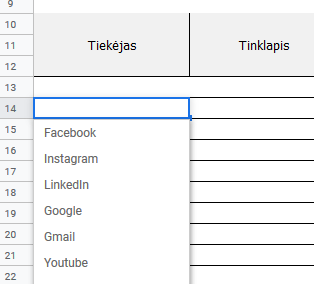
\includegraphics[scale=0.7]{Images/Screenshots/records-dropdown-list.PNG}
    \caption{Pasirenkamasis sąrašas}
    \label{img:model}
\end{figure}

\begin{figure}[H]
    \centering
    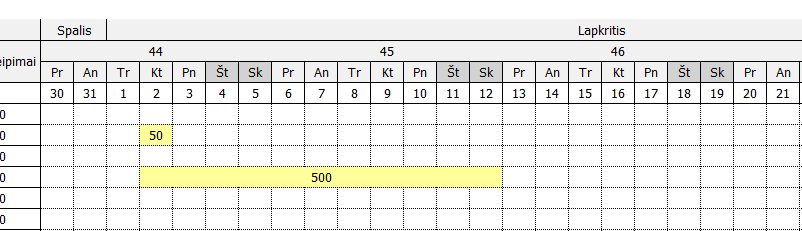
\includegraphics[scale=0.7]{Images/Screenshots/records-calendar.PNG}
    \caption{Kalendoriaus reikšmės}
    \label{img:model}
\end{figure}

\subsection{Užsakymo kūrimas}
Užsakymo kūrimas yra kita pagrindinė užduotis. Ją galima atlikti tik užbaigus Media plano kūrimą. Ji skirta sugeneruoti konkretaus kanalo sumažintą Media plano versiją.

\bigskip
Užsakymo kūrimo instrukcijos: 
\begin{enumerate}
    \itemsep0em 
    \item Nueiti į Media plano skaičiuoklės lapą;
    \item Paspausti ant meniu pasirinkimo „Šablonai“ (žr. 1 pav.);
    \item Paspausti ant sub-meniu pasirinkimo „Užsakymo šablonas“ (žr. 2 pav.);
    \item Palaukti, kol atsidarys dialogo langas (modalas) (žr. 16 pav.);
    \item Pasirinkti norimą Užsakymo kalbą (žr. 16 pav.);
    \item Pasirinkti norimą Užsakymo kanalą (žr. 16 pav.);
    \item Paspausti mygtuką „Kurti užsakymą“ (žr. 16 pav.);
    \item Palaukti, kol bus įvykdytas programinis kodas, t.y. sukuriamas naujas skaičiuoklės lapas pavadinimu „Order *kanalo pavadinimas*“ (žr. 17 pav.). 
\end{enumerate}

\bigskip
Rekomendacijos:
\begin{itemize}
    \itemsep0em 
    \item Užsakymas gali būti kuriamas tik iš Media plano;
    \item Prieš kuriant Užsakymą reikia turėti užpildytą bent vieną įrašų eilutę;
    \item Sugeneruotame Užsakyme visos reikšmės paimtos iš Media plano atitinkamų eilučių, todėl nerekomenduojama nieko keisti;
    \item 4 punktas. Norint išeiti iš dialogo lango, paspausti mygtuką „Uždaryti“ (žr. 16 pav.);
    \item 5 punktas. Numatytoji kalba - lietuvių (LT), tačiau galima pasirinkti ir anglų kalbą (EN) (žr. 16 pav.);
    \item 6 punktas. Numatytasis kanalas - pirmas nuo viršaus, tačiau galima rinktis ir kitas reikšmes iš pasirenkamojo sąrašo (žr. 16 pav.);
    \item Rekomenduotina, kad viename skaičiuoklės faile būtų tik vienas to pačio kanalo Užsakymas. Jeigu reikia 2 ar daugiau to paties kanalo užsakymų, patartina pervadinti anksčiau sukurtą užsakymą.
\end{itemize}

\bigskip
Galimos problemos:
\begin{itemize}
    \itemsep0em 
    \item 3 punktas. Paspaudus mygtuką „Užsakymo šablonas“ atsidaro pranešimas (žr. 18 pav.). Tokiu atveju reikia paspausti „Ok“. Tai reiškia, kad funkcija buvo kviesta ne iš Media plano skaičiuoklės lapo. Nueikite į Media plano skaičiuoklės lapą ir bandykite pakartoti viską nuo 1 punkto;
    \item 7 punktas. Paspaudus mygtuką „Užsakymo šablonas“ atsidaro pranešimas (žr. 19 pav.). Tokiu atveju reikia paspausti „Ok“. Tai reiškia, kad Užsakymo skaičiuoklės lapas konkrečiam kanalui jau yra sukurtas. Tokiu atveju rekomenduotina pervadinti esamą užsakymą ir bandyti viską atlikti nuo 1 punkto;
    \item 7 punktas. Paspaudus mygtuką „Užsakymo šablonas“ nieko nevyksta. Taip gali nutikti retais atvejais. Rekomenduotina pabandyti viską atlikti nuo 1 punkto, tik gerokai lėčiau. 
\end{itemize}

\begin{figure}[H]
    \centering
    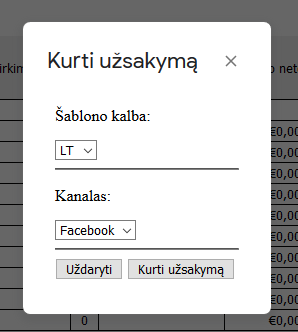
\includegraphics[scale=0.7]{Images/Screenshots/modal-order.PNG}
    \caption{Užsakymo kūrimo dialogas}
    \label{img:model}
\end{figure}

\begin{figure}[H]
    \centering
    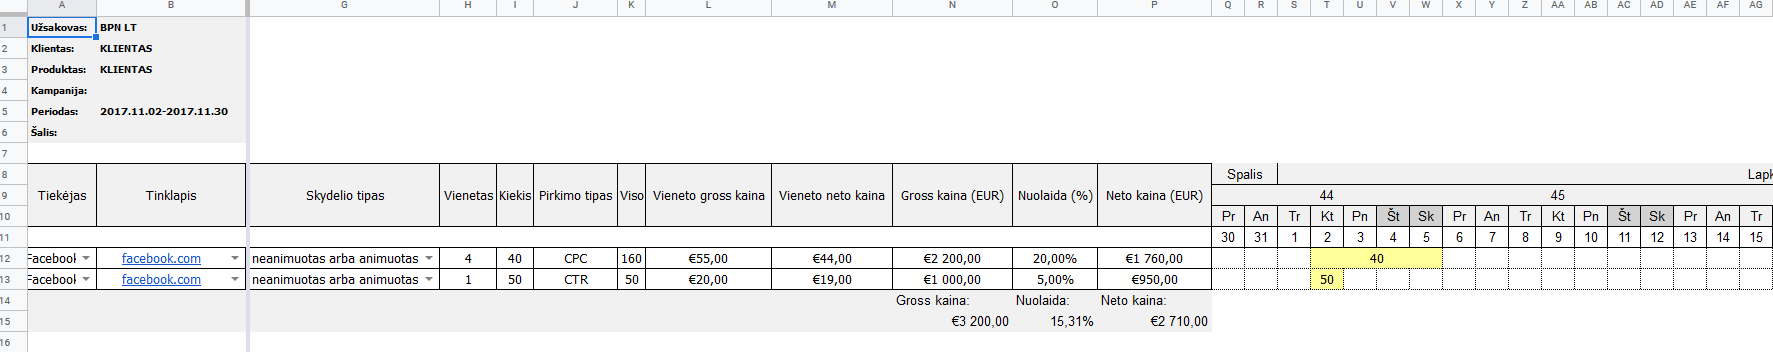
\includegraphics[scale=0.35]{Images/Screenshots/generated-order.PNG}
    \caption{Sugeneruotas Užsakymo šablonas}
    \label{img:model}
\end{figure}

\begin{figure}[h]
    \centering
    \begin{minipage}{0.45\textwidth}
        \centering
        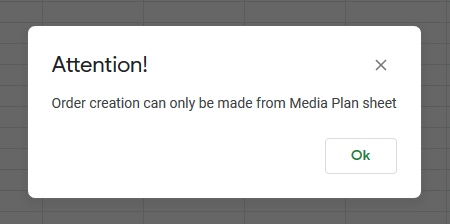
\includegraphics[scale=0.6]{Images/Screenshots/order-alert.PNG} 
        \caption{Užsakymo kūrimo klaida \#1}
    \end{minipage}\hfill
    \begin{minipage}{0.45\textwidth}
        \centering
        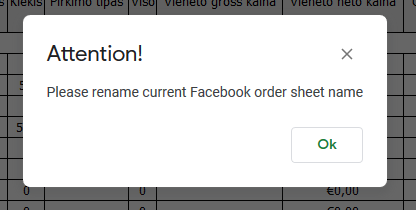
\includegraphics[scale=0.6]{Images/Screenshots/modal-order-alert.PNG}
        \caption{Užsakymo kūrimo klaida \#2}
    \end{minipage}
\end{figure}

\subsection{Media plano užbaigimas}
Media plano užbaigimas yra pagalbinė užduotis. Ją galima atlikti tik užbaigus Media plano kūrimą. Ji skirta sugeneruoti Media plano parašą.

\bigskip
Įrašų generavimo instrukcijos: 
\begin{enumerate}
    \itemsep0em 
    \item Nueiti į Media plano skaičiuoklės lapą;
    \item Paspausti ant meniu pasirinkimo „Parankiniai“ (žr. 1 pav.);
    \item Paspausti ant sub-meniu pasirinkimo „Užbaigti šabloną“ (žr. 3 pav.);
    \item Palaukti, kol bus sugeneruotas parašas (žr. 20 pav.);
    \item Įvesti atitinkamas reikšmes į parašo laukus.
\end{enumerate}

\bigskip
Rekomendacijos:
\begin{itemize}
    \itemsep0em 
    \item Atlikti užduotį tada, kai visi Media plano laukai bus užpildyti ir bus aišku, kad tai galutinis variantas;
    \item Prieš atliekant užduotį galutinai žinoti periodą, nes „Vėliausias patvirtinimas iki“ generuojamas pagal formulę: periodo pradžios data - 1 diena (žr. 20 pav.);
    \item Parašo pozicija yra 4 eilutėmis žemiau, negu paskutinė netuščia eilutė (žr. 20 pav.).
\end{itemize}

\bigskip
Galimos problemos:
\begin{itemize}
    \itemsep0em 
    \item Nenumatyta
\end{itemize}

\begin{figure}[H]
    \centering
    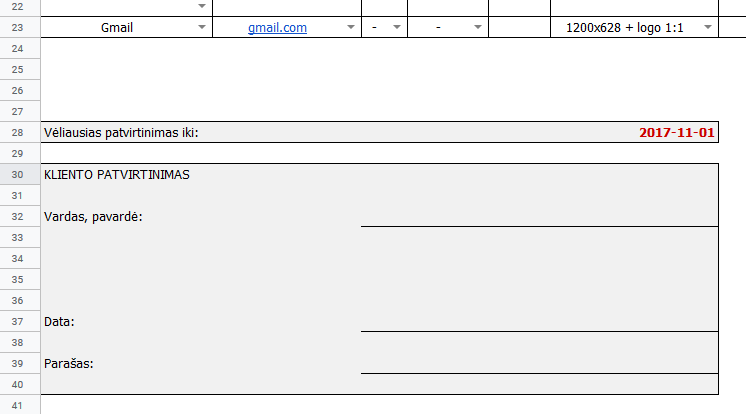
\includegraphics[scale=0.5]{Images/Screenshots/signature.PNG}
    \caption{Media plano sugeneruotas parašas}
    \label{img:model}
\end{figure}





%----------------------------------------------------------------------------------------
%	T E C H N I N Ė      D O K U M E N T A C I J A
%----------------------------------------------------------------------------------------


\pagebreak
\section{Techninė dokumentacija}

\subsection{Užduočių diagramos}
Užduočių diagramos naudingos suvokti projekto vadovo tikslus ir visas veiklas, kurias jis gali vykdyti projekto srityje (angl. \textit{Scope}).

\subsubsection {Visi agentai ir užduotys}
Žemiau pateiktame paveikslėlyje (žr. 1 pav.) pavaizduoti visi su Skaitmeninės reklamos planavimo optimizavimo projektu susiję agentai bei sugrupuotos užduotys. Projekto agentas kol kas yra vienintelis - projekto vadovas, Veiklos suskirstytos į šablonų kūrimus ir pagalbinius įrankius, skirtus sėkmingai šablonų realizacijai.

\begin{figure}[H]
    \centering
    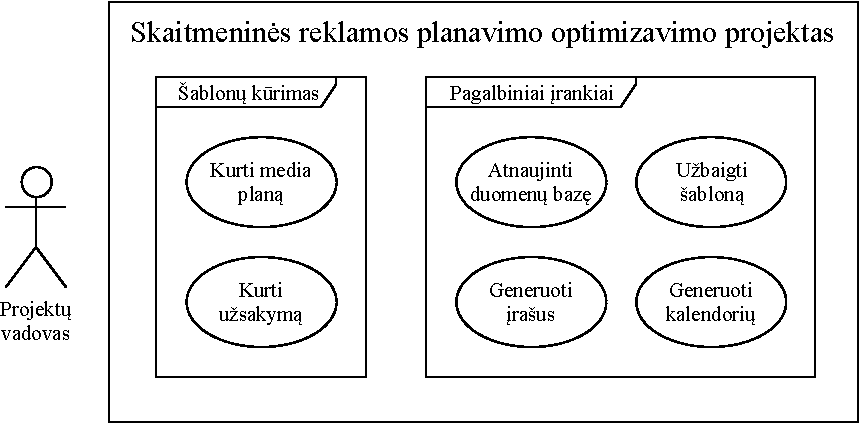
\includegraphics[scale=0.9]{Images/agents-use-cases.pdf}
    \caption{Visi agentai ir užduotys}
    \label{img:model}
\end{figure}

\subsubsection {Media plano kūrimas}
Šioje diagramoje pavaizduotas „Media plano kūrimas“ (žr. 2 pav.). Projektų vadovui pasirinkus šią užduotį jis toliau gali rinktis tolimesnius scenarijus, tokius kaip „Atnaujinti duomenų bazę“, „Generuoti kalendorių“, „Generuoti įrašus“, „Kurti užsakymą“ bei „Užbaigti šabloną“. Visi šie pasirinkimai projektų vadovui būtų neprieinami, jeigu jis prieš tai nebūtų pasirinkęs „Kurti media planą“.

\begin{figure}[H]
    \centering
    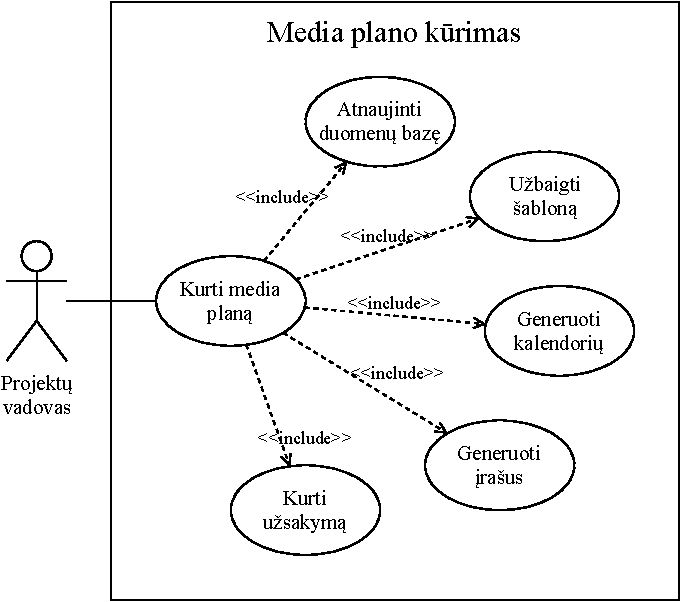
\includegraphics[scale=0.95]{Images/use-case-media-plan.pdf}
    \caption{Media plano kūrimo užduotis}
    \label{img:model}
\end{figure}

\subsubsection {Užsakymo kūrimas}
Trečioje užduočių diagramoje (žr. 3 pav.) vaizduojamas „Užsakymo kūrimas“. Projekto vadovas, atlikęs užduotį „Media plano kūrimas“, gali atlikti užduotį „Kurti užsakymą“. Užduotis „Kurti užsakymą“ turi 2 atmainas: „Kurti užsakymą lietuvių kalba“ ir „Kurti užsakymą anglų kalba“. Atlikus vieną iš šių užduočių, automatiškai įvykdomos užduotys „Kopijuoti įrašus“ ir „Generuoti kalendorių“.

\begin{figure}[H]
    \centering
    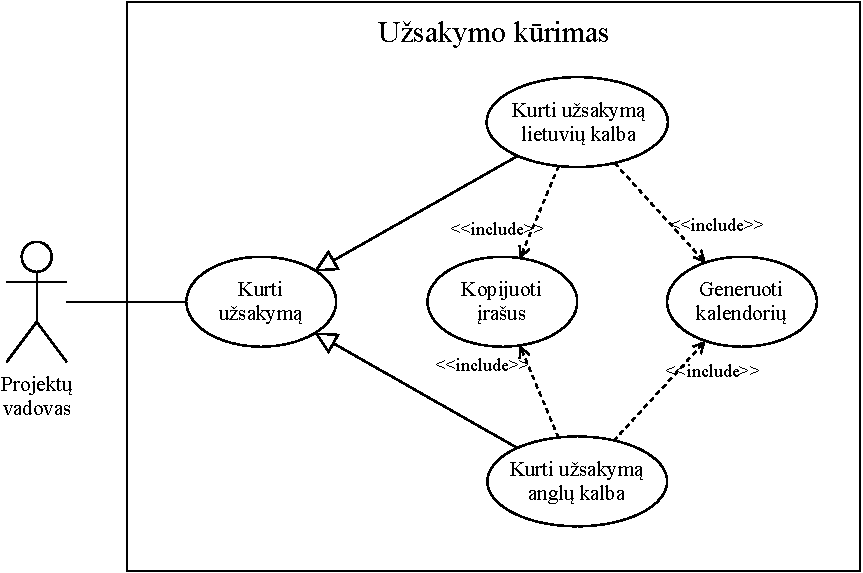
\includegraphics[scale=0.85]{Images/use-case-order.pdf}
    \caption{Užsakymo kūrimo užduotis}
    \label{img:model}
\end{figure}

\subsection{Klasių/modulių diagramos}
Projekto klasių arba modulių diagramos turėtų padėti suprasti funkcijų grupavimo tikslus ir kriterijus, be to, sužinoti, kur galima pasiekti konkrečius metodus bei įgyvendintą funkcionalumą.

\subsubsection{Bendra modulių diagrama}
Žemiau pateikiama diagrma su visais Google Apps Script (.gs) ir HTML (.html) failais ir juose esančiomis funkcijomis (žr. 4 pav.). Kiekvienas modulis - failas nagrinėjamas atskirai atitinkamuose poskyriuose.

\begin{figure}[H]
    \centering
    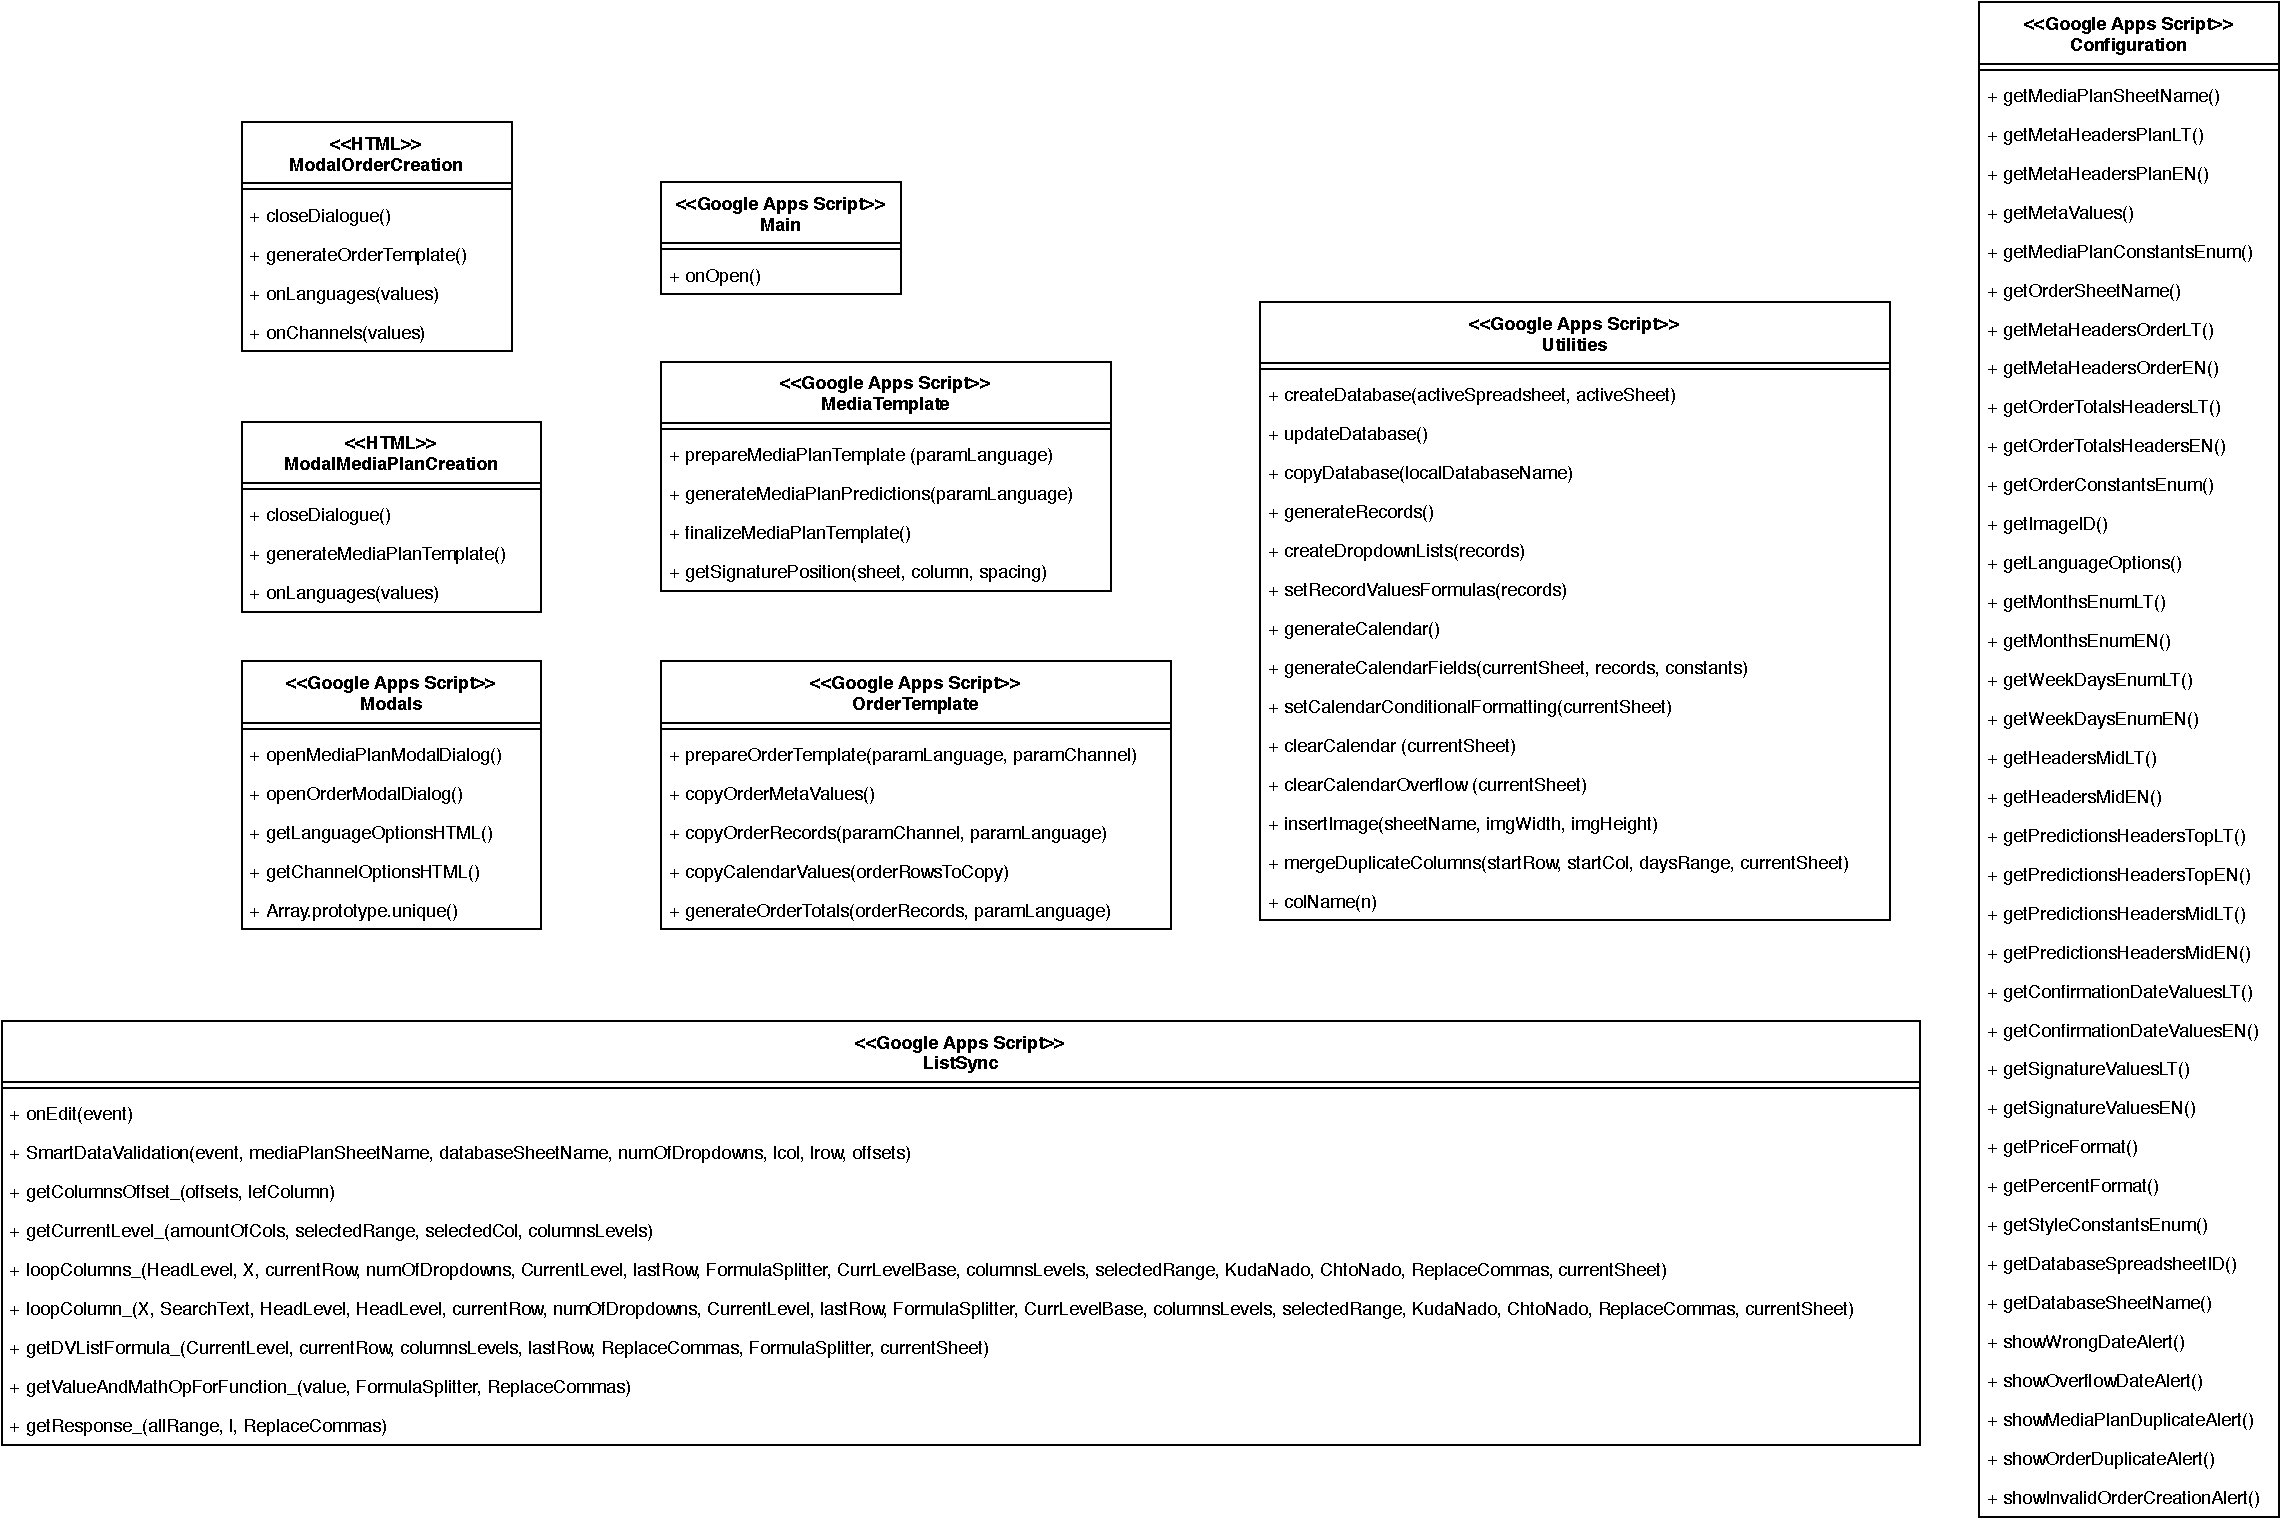
\includegraphics[scale=0.35]{Images/modules.pdf}
    \caption{Bendra modulių diagrama}
    \label{img:model}
\end{figure}

\subsubsection{Modulis „Main“}
Modulis „Main“ (žr. 5 pav.) turi vienintelę funkciją „onOpen()“. Ši funkcija yra skirta sugeneruoti individualius meniu pasirinkimus, kurių įprastoje Google Sheets naršyklės aplikacijoje neaptiktumėme. „onOpen()“ yra viena iš Google Apps Script rezervuotų funkcijų, kuri pradedama vykdyti atidarius arba perkrovus Google Sheets lapą, taigi pati pirma, kuri įvykdoma.

\begin{figure}[H]
    \centering
    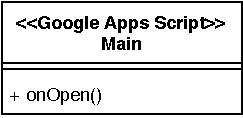
\includegraphics[scale=1]{Images/module-main.pdf}
    \caption{Modulis „Main“}
    \label{img:model}
\end{figure}

\subsubsection{Modulis „Modals“}
Modulis „Modals“ (žr. 6 pav.) skirtas darbui su modalais - iššokančiais langais su pasirinkimais. Funkcijos šiame modulyje skirtos modalų atidarymui bei reikšmių juose supildymui.

\begin{figure}[H]
    \centering
    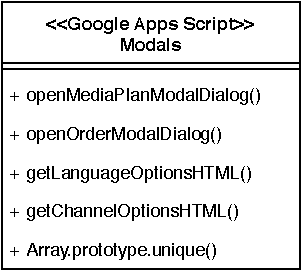
\includegraphics[scale=0.8]{Images/module-modals.pdf}
    \caption{Modulis „Modals“}
    \label{img:model}
\end{figure}

\subsubsection{Modulis „ModalMediaPlanCreation“}
Modulis „ModalMediaPlanCreation“ (žr. 7 pav.) yra HTML failas, atvaizduojantis Media plano kūrimo modalą. Jis savyje turi JavaScript funkcijas, naudojamas modalo uždarymui, reikšmių modale supildymui bei Media plano skaičiuoklės sukūrimui.

\begin{figure}[H]
    \centering
    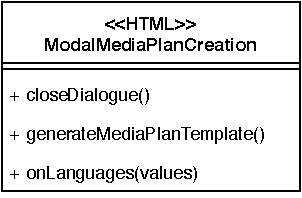
\includegraphics[scale=0.8]{Images/module-modal-media-plan-creation.pdf}
    \caption{Modulis „ModalMediaPlanCreation“}
    \label{img:model}
\end{figure}

\subsubsection{Modulis „ModalOrderCreation“}
Modulis „ModalOrderCreation“ (žr. 8 pav.) yra HTML failas, atvaizduojantis užsakymo kūrimo modalą. Jis savyje turi JavaScript funkcijas, naudojamas modalo uždarymui, reikšmių modale supildymui bei Užsakymo skaičiuoklės sukūrimui.

\begin{figure}[H]
    \centering
    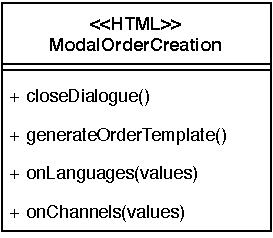
\includegraphics[scale=0.8]{Images/module-modal-order-creation.pdf}
    \caption{Modulis „ModalOrderCreation“}
    \label{img:model}
\end{figure}

\subsubsection{Modulis „MediaTemplate“}
Modulis „MediaTemplate“ (žr. 9 pav.) skirtas generuoti visam baziniam Media plano apipavidalinimui: stulpelių ir langelių reikšmėms, stiliams, spalvoms, ir t.t. Taip pat projektų vadovui užbaigus Media plano pildymą sugeneruoti parašą.

\begin{figure}[H]
    \centering
    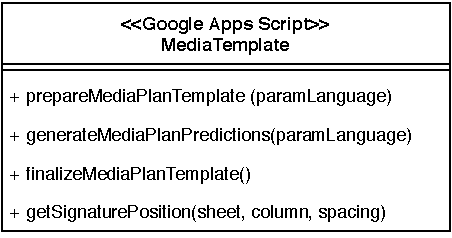
\includegraphics[scale=0.8]{Images/module-media-template.pdf}
    \caption{Modulis „MediaTemplate“}
    \label{img:model}
\end{figure}

\subsubsection{Modulis „OrderTemplate“}
Modulis „OrderTemplate“ (žr. 10 pav.) skirtas generuoti užsakymą pagal pasirinktą kanalą. Sugeneruojamas bazinis apipavidalinimas, tačiau jis atsiranda nukopijavus apipavidalinimą tiesiogiai iš tam tikrų Media plano laukų. Iš Media plano nekopijuojama tik su kainų suma susijusios reikšmės.

\begin{figure}[H]
    \centering
    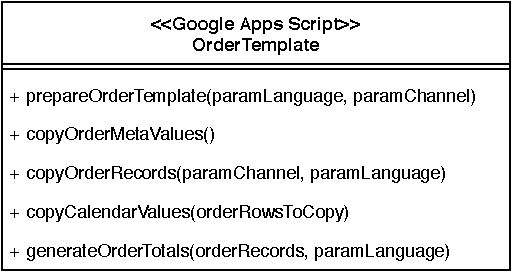
\includegraphics[scale=0.7]{Images/module-order-template.pdf}
    \caption{Modulis „OrderTemplate“}
    \label{img:model}
\end{figure}

\subsubsection{Modulis „Utilities“}
Modulis „Utilities“ (žr. 11 pav.) skirtas visoms pagalbinėms funkcijoms, kurias naudoja tiek Media planas, tiek Užsakymas. Visas funkcijas būtų galima sugrupuoti į 4 kategorijas: duomenų bazės, įrašų, kalendoriaus bei neapibrėžtas. 

Duomenų bazės kategorijos funkcijos atsakingos už duomenų bazės sukūrimą, atnaujinimą ir sinchronizavimą su darbo skaičiuokle. 

Įrašų kategorijoje funkcijos atsakingos už naujų eilučių su pasirinkimų sąrašais generavimui, formulių ir formatų tose eilutėse nustatymui.

Kalendoriaus kategorijos funkcijos skirtos kalendoriaus generavimui, formatui kalendoriaus laukuose nustatymui.

Neapibrėžtų funkcijų kategorijoje galime išvysti tokius metodus, kaip paveikslėlio į skaičiuoklę įterpimą arba kitoms funkcijoms reikalingus metodus, t.y. laukų sujungimui (angl. \textit{Merge}) bei stulpelių numerių pavertimui į raidinį formatą.

\begin{figure}[H]
    \centering
    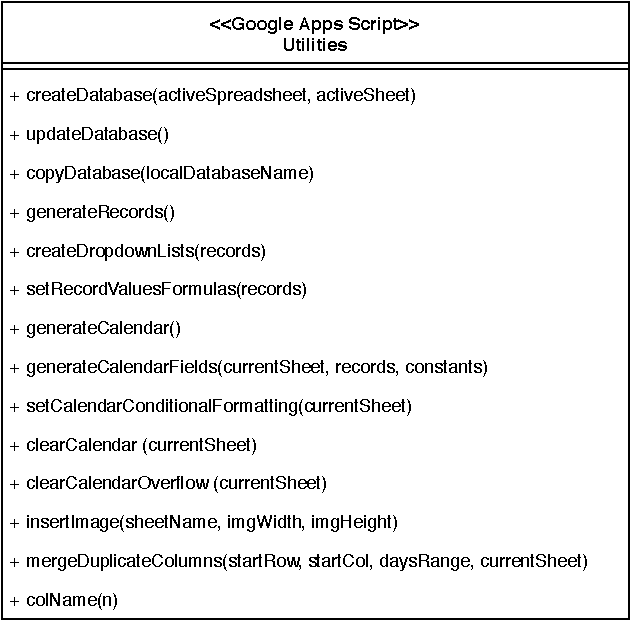
\includegraphics[scale=0.6]{Images/module-utilities.pdf}
    \caption{Modulis „Utilities“}
    \label{img:model}
\end{figure}

\subsubsection{Modulis „ListSync“}
Modulis „ListSync“ (žr. 12 pav.) yra funkcijų visuma, skirta dinamiškam pasirenkamųjų sąrašų įgyvendinimui. Kadangi ši implementacija nėra lengva ir triviali, buvo pasitelkti internetiniai šaltiniai, o konkrečiai - vienas sprendimas su tam tikromis projekto autoriaus asmeniniu sprendimu pritaikytomis korekcijomis\footnote{https://gist.github.com/Max-Makhrov/060c21da4f280b6faac82337dadb16e5}. Kadangi sprendimas yra sudėtingas, jam buvo išskirtas atskiras modulis.

\begin{figure}[H]
    \centering
    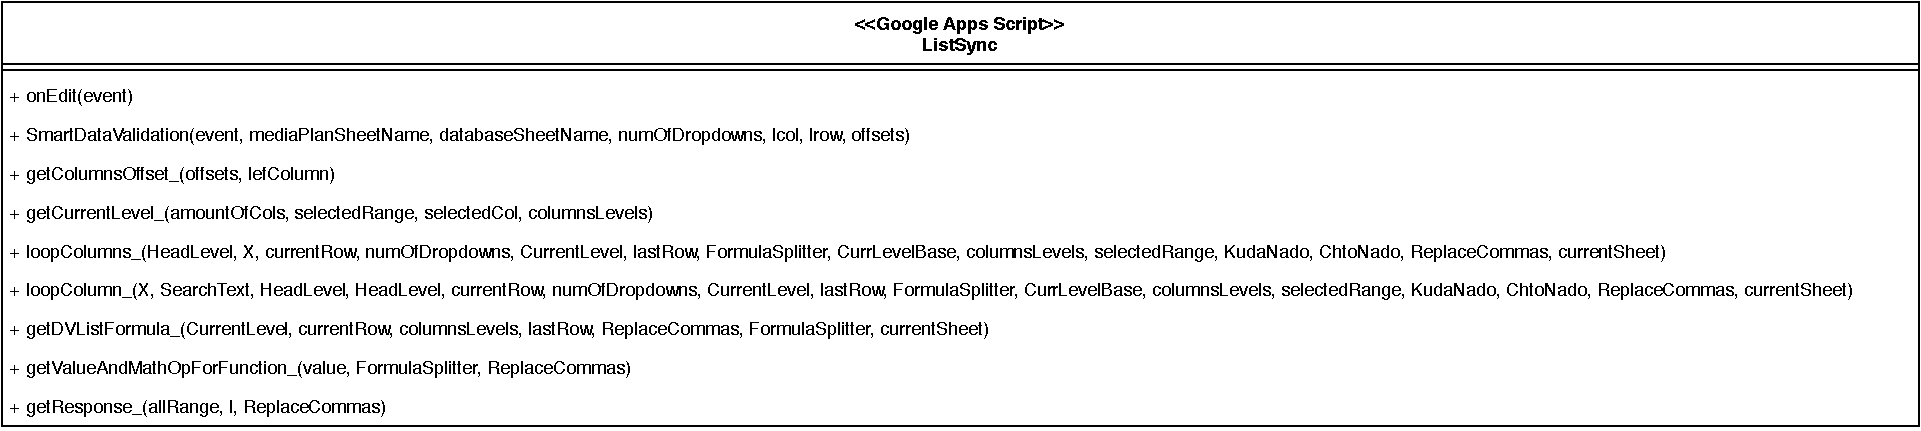
\includegraphics[scale=0.5]{Images/module-list-sync.pdf}
    \caption{Modulis „ListSync“}
    \label{img:model}
\end{figure}

\subsubsection{Modulis „Configuration“}
Modulį „ListSync“ (žr. 13 pav.) galima interpretuoti kaip konfigūracinį failą. Jame įvykdyti pakeitimai atsispindės visame projekte, todėl su pakeitimais šiame modulyje reikia elgtis itin atsakingai ir atsargiai. Šiame modulyje esančios funkcijos skirtos apibrėžti konstantinėms skaitinėms ir langelių reikšmėms, spalvoms, nuorodoms į kitus failus ir t.t.

Modulyje taip pat yra metodai, skirti iššokantiesiems įspėjamiesiems pranešimams vaizduoti.

\begin{figure}[H]
    \centering
    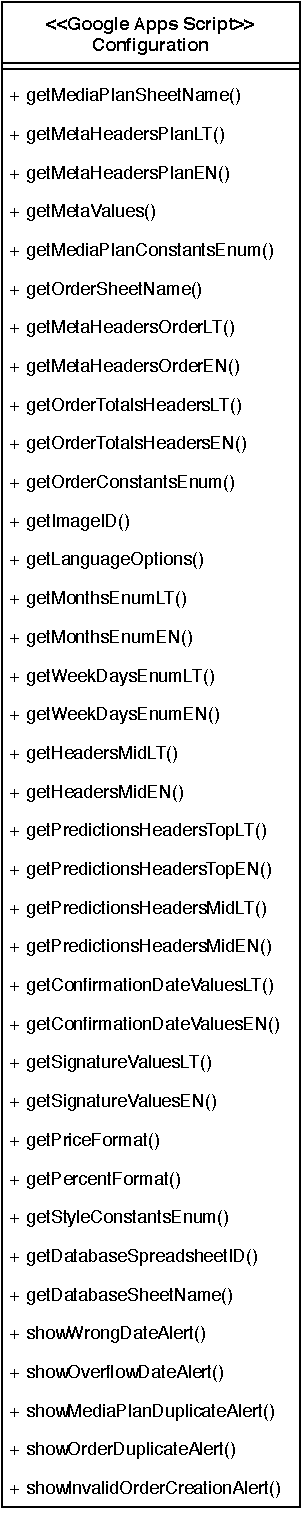
\includegraphics[scale=0.5]{Images/module-configuration.pdf}
    \caption{Modulis „Configuration“}
    \label{img:model}
\end{figure}

\subsection{Sekų diagramos}
„“





%----------------------------------------------------------------------------------------
%	P R O G R A M I N I O      K O D O      D O K U M E N T A C I J A
%----------------------------------------------------------------------------------------


\subsection{Programinio kodo dokumentacija}


%----------------------------------------------------------------------------------------
%	Main
%----------------------------------------------------------------------------------------

\subsubsection{Modulis „Main“}

\textit{\textbf{onOpen()}} - Google Apps Script rezervuota funkcija su kustomizuotu įgyvendinimu. Funkcija kviečiama atidarius arba perkrovus skaičiuoklės dokumentą. 

\bigskip
\textit{Vykdymo seka}:
\begin{enumerate}
    \itemsep0em 
    \item Nustatomi pagrindinio meniu pasirinkimai;
    \item Nustatomi pagrindinio meniu sub-meniu pasirinkimai ir priskiriamos jų funkcijų reikšmės;
    \item Priskiriamos vidinės konstantinės skaičiuoklės reikšmės.
\end{enumerate}


%----------------------------------------------------------------------------------------
%	Modals
%----------------------------------------------------------------------------------------

\subsubsection{Modulis „Modals“}

\textit{\textbf{openMediaPlanModalDialog()}} - funkcija, skirta Media plano modalo atidarymui. Funkcija kviečiama iš meniu pasirinkimo.

\bigskip
\textit{Vykdymo seka}:
\begin{enumerate}
    \itemsep0em 
    \item Sukuriamas HTML failas \textit{ModalMediaPlanCreation.html} pagrindu;
    \item Nustatomas modalo dydis ir antraštė;
    \item Modalas atvaizduojamas vartotojui.
\end{enumerate}

\bigskip
\textit{\textbf{openOrderModalDialog()}} - funkcija, skirta Užsakymo modalo atidarymui. Funkcija kviečiama iš meniu pasirinkimo.

\bigskip
\textit{Vykdymo seka}:
\begin{enumerate}
    \itemsep0em 
    \item Patikrinama, ar funkcija iškviesta iš Media plano skaičiuoklės lapo. Jei ne - parodomas pranešimas ir nustojama vykdyti;
    \item Sukuriamas HTML failas \textit{ModalOrderCreation.html} pagrindu;
    \item Nustatomas modalo dydis ir antraštė;
    \item Modalas atvaizduojamas vartotojui.
\end{enumerate}

\bigskip
\textit{\textbf{getLanguageOptionsHTML()}} - funkcija, skirta perduoti kalbų pasirinkimo duomenis modalams. 
Funkcija kviečiama iš \textit{ModalMediaPlanCreation.html} ir \textit{ModalOrderCreation.html} modulių.

\bigskip
\textit{Vykdymo seka}:
\begin{enumerate}
    \itemsep0em 
    \item Grąžina kalbų pasirinkimo sąrašą kviečiant \textit{Configuration} modulio funkciją.
\end{enumerate}

\bigskip
\textit{\textbf{getChannelOptionsHTML()}} - funkcija, skirta perduoti kanalų pasirinkimo duomenis modalams. 
Funkcija kviečiama iš \textit{ModalOrderCreation.html} modulio.

\bigskip
\textit{Vykdymo seka}:
\begin{enumerate}
    \itemsep0em 
    \item Pasirenkami visi Media plano kanalai;
    \item Vykdomas algoritmas, atrinktis unikalius kanalus iš visų kanalų masyvo;
    \item Grąžinamas unikalių kanalų masyvas.
\end{enumerate}

\bigskip
\textit{\textbf{Array.prototype.unique()}} - funkcija, skirta atrinkti unikalias masyvo reikšmes. 
Funkcija kviečiama iš \textit{Modals.gs} modulio \textit{getChannelOptionsHTML()} funkcijos.


%----------------------------------------------------------------------------------------
%	ModalMediaPlanCreation
%----------------------------------------------------------------------------------------

\subsubsection{Modulis „ModalMediaPlanCreation“}

\textit{\textbf{window.closeDialogue()}} - funkcija, skirta uždaryti modalo langą. Funkcija kviečiama iš modalo lango pasirinkus mygtuką \textit{Uždaryti}.

\bigskip
\textit{\textbf{window.generateMediaPlanTemplate()}} - funkcija, skirta inicijuoti Media plano kūrimą. Funkcija kviečiama iš modalo lango pasirinkus mygtuką \textit{Kurti Media planą}.

\bigskip
\textit{Vykdymo seka}:
\begin{enumerate}
    \itemsep0em 
    \item Paimama pasirinkta Media plano kalba;
    \item Kviečiama Media plano kūrimo funkcija;
    \item Modalas uždaromas.
\end{enumerate}

\bigskip
\textit{\textbf{window.onLanguages(languages)}} - funkcija, skirta užpildyti modale esančius kalbų pasirinkimus. Funkcija kviečiama iškart atidarius modalą.

\bigskip
\textit{Parametrai}:
\begin{itemize}
    \itemsep0em 
    \item \textit{languages} - kalbų, kurias vartotojas galės rinktis, masyvas.
\end{itemize}


%----------------------------------------------------------------------------------------
%	ModalOrderCreation
%----------------------------------------------------------------------------------------

\subsubsection{Modulis „ModalOrderCreation“}

\textit{\textbf{window.closeDialogue()}} - funkcija, skirta uždaryti modalo langą. Funkcija kviečiama iš modalo lango pasirinkus mygtuką \textit{Uždaryti}.

\bigskip
\textit{\textbf{window.generateOrderTemplate()}} - funkcija, skirta inicijuoti Užsakymo kūrimą. Funkcija kviečiama iš modalo lango pasirinkus mygtuką \textit{Kurti Užsakymą}.

\bigskip
\textit{Vykdymo seka}:
\begin{enumerate}
    \itemsep0em 
    \item Paimama pasirinkta Užsakymo kalba;
    \item Paimamas pasirinkta Užsakymo kanalas;
    \item Kviečiama Užsakymo kūrimo funkcija;
    \item Modalas uždaromas.
\end{enumerate}

\textit{\textbf{window.onLanguages(languages)}} - funkcija, skirta užpildyti modale esančius kalbų pasirinkimus. Funkcija kviečiama iškart atidarius modalą.

\bigskip
\textit{Parametrai}:
\begin{itemize}
    \itemsep0em 
    \item \textit{languages} - kalbų, kurias vartotojas galės rinktis, masyvas.
\end{itemize}

\bigskip
\textit{\textbf{window.onChannels(channels)}} - funkcija, skirta užpildyti modale esančius kanalų pasirinkimus. Funkcija kviečiama iškart atidarius modalą.

\bigskip
\textit{Parametrai}:
\begin{itemize}
    \itemsep0em 
    \item \textit{channels} - kanalų, kuriuos vartotojas galės rinktis, masyvas.
\end{itemize}


%----------------------------------------------------------------------------------------
%	MeiaPlanTemplate
%----------------------------------------------------------------------------------------

\subsubsection{Modulis „MediaTemplate“}

\textit{\textbf{prepareMediaPlanTemplate(paramLanguage)}} - funkcija, skirta sukurti Media planą. Funkcija kviečiama iš \textit{ModalMediaPlanCreation.gs} modulio \textit{window.generateMediaPlan Template()} funkcijos.

\bigskip
\textit{Parametrai}:
\begin{itemize}
    \itemsep0em 
    \item \textit{paramLanguage} - kalba, kuria kuriamas media planas.
\end{itemize}

\bigskip
\textit{Vykdymo seka}:
\begin{enumerate}
    \itemsep0em 
    \item Patikrinama, ar Media plano bei lokalios duomenų bazės yra sukurtos.
    \begin{itemize}
    \itemsep0em 
        \item Jeigu abi nėra nesukurtos - sukuriamos;
        \item Jeigu Media planas yra sukurtas - parodomas pranešimas ir nustojama vykdyti;
        \item Jeigu duomenų bazė yra sukurta - nieko nedaroma.
    \end{itemize}
    \item Priklausomai nuo \textit{paramLanguage} parametro, nustatoma skaičiuoklės ir jos laukų kalba;
    \item Nustatomos numatytųjų langelių reikšmės;
    \item Nustatomi numatytųjų langelių stiliai;
    \item Įterpiamas BPN logotipas.
\end{enumerate}

\bigskip
\textit{\textbf{generateMediaPlanPredictions(paramLanguage)}} - funkcija, skirta sukurti Media plano papildomus prognozės stulpelius. Funkcija kviečiama iš \textit{MediaPlanTemplate.gs} modulio \textit{prepareMediaPlanTemplate(paramLanguage)} funkcijos.

\bigskip
\textit{Parametrai}:
\begin{itemize}
    \itemsep0em 
    \item \textit{paramLanguage} - kalba, kuria kuriamos media plano prognozės.
\end{itemize}

\bigskip
\textit{Vykdymo seka}:
\begin{enumerate}
    \itemsep0em 
    \item Priklausomai nuo \textit{paramLanguage} parametro, nustatoma prognozių laukų kalba;
    \item Nustatomos numatytųjų langelių reikšmės;
    \item Nustatomi numatytųjų langelių stiliai.
\end{enumerate}

\bigskip
\textit{\textbf{finalizeMediaPlanTemplate()}} - funkcija, skirta užbaigti Media planą sukuriant parašą. Funkcija kviečiama iš meniu pairinkimo.

\bigskip
\textit{Vykdymo seka}:
\begin{enumerate}
    \itemsep0em 
    \item Patikrinama, ar funkcija buvo iškviesta iš Media plano skaičiuoklės lapo;
    \item Patikrinama Media plano skaičiuoklės lapo kalba;
    \item Nustatomos parašo numatytųjų langelių reikšmės;
    \item Nustatomi numatytųjų langelių stiliai.
\end{enumerate}


%----------------------------------------------------------------------------------------
%	OrderTemplate
%----------------------------------------------------------------------------------------

\subsubsection{Modulis „OrderTemplate“}

\textit{\textbf{prepareOrderTemplate(paramLanguage, paramChannel)}} - funkcija, skirta sukurti konkretaus kanalo Užsakymą. Funkcija kviečiama iš \textit{ModalOrderCreation.gs} modulio \textit{window.generateOrderTemplate()} funkcijos.

\bigskip
\textit{Parametrai}:
\begin{itemize}
    \itemsep0em 
    \item \textit{paramLanguage} - kalba, kuria kuriamas Užsakymas;
    \item \textit{paramChannel} - kanalas, kuriam kuriamas Užsakymas.
\end{itemize}

\bigskip
\textit{Vykdymo seka}:
\begin{enumerate}
    \itemsep0em 
    \item Patikrinama, ar toks pats Užsakymo skaičiuoklės lapas jau egzistuoja. Jei egzistuoja - parodomas pranešimas ir funkcijos vykdymas nutraukiamas. Jei neegzistuoja - funkcijos vykdymas tęsiamas;
    \item Priklausomai nuo \textit{paramLanguage} parametro, nustatoma skaičiuoklės lapo ir jos laukų kalba;
    \item Nustatomos numatytųjų langelių reikšmės;
    \item Nustatomi numatytųjų langelių stiliai;
    \item Įterpiamas BPN logotipas;
    \item Sukuriamas kalendorius;
    \item Nukopijuojamos su Užsakymo kanalu susijusios reikšmės iš Media plano į Užsakymą.
\end{enumerate}

\bigskip
\textit{\textbf{copyOrderMetaValues()}} - funkcija, skirta nukopijuoti Užsakymui reikalingas Meta reikšmes. Funkcija kviečiama iš \textit{OrderTemplate.gs} modulio \textit{prepareOrderTemplate(param Language, paramChannel))} funkcijos.

\bigskip
\textit{Vykdymo seka}:
\begin{enumerate}
    \itemsep0em 
    \item Nustatomi Media plano ir Užsakymo Meta reikšmių langelių intervalai;
    \item Media plano Meta reikšmių langelių intervalo reikšmės nukopijuojamos į Užsakymo Meta reikšmių langelių intervalą.
\end{enumerate}

\bigskip
\textit{\textbf{copyOrderRecords(paramChannel, paramLanguage)}} - funkcija, skirta nukopijuoti Užsakymui reikalingas reikšmes. Funkcija kviečiama iš \textit{OrderTemplate.gs} modulio \textit{prepareOrderTemplate(paramLanguage, paramChannel)} funkcijos.

\bigskip
\textit{Parametrai}:
\begin{itemize}
    \itemsep0em 
    \item \textit{paramLanguage} - kalba, kuria kuriamas Užsakymas;
    \item \textit{paramChannel} - kanalas, kuriam kuriamas Užsakymas.
\end{itemize}

\bigskip
\textit{Vykdymo seka}:
\begin{enumerate}
    \itemsep0em 
    \item Nustatomos Media plano eilutės, kurias reikia kopijuoti;
    \item Atitinkamos eilutės nukopijuojamos iš Media plano į Užsakymo skaičiuoklės lapą;
    \item Generuojami individualaus Užsakymo galutiniai rodikliai;
    \item Kopijuojamos kalendoriaus reikšmės.
\end{enumerate}

\bigskip
\textit{\textbf{copyCalendarValues(orderRowsToCopy)}} - funkcija, skirta nukopijuoti Užsakymui reikalingas kalendoriaus reikšmes. Funkcija kviečiama iš \textit{OrderTemplate.gs} modulio \textit{copyOrderRecords(paramChannel, paramLanguage)} funkcijos.

\bigskip
\textit{Parametrai}:
\begin{itemize}
    \itemsep0em 
    \item \textit{orderRowsToCopy} - eilučių numerių masyvas, kuriuos reikia kopijuoti iš Media plano į Užsakymo skaičiuoklės lapą.
\end{itemize}

\bigskip
\textit{Vykdymo seka}:
\begin{enumerate}
    \itemsep0em 
    \item Nustatomas Media plano ir Užsakymo kalendoriaus reikšmių langelių intervalai;
    \item Media plano langelių intervalo reikšmės nukopijuojamos į Užsakymo kalendoriaus reikšmių langelių intervalą.
\end{enumerate}

\bigskip
\textit{\textbf{generateOrderTotals(orderRecords, paramLanguage)}} - funkcija, skirta generuoti Užsakymui reikalingas galutines rodiklių reikšmes. Funkcija kviečiama iš \textit{OrderTemplate.gs} modulio \textit{copyOrderRecords(paramChannel, paramLanguage)} funkcijos.

\bigskip
\textit{Parametrai}:
\begin{itemize}
    \itemsep0em 
    \item \textit{orderRecords} - eilučių, kurios buvo nukopijuotos iš Media plano į Užsakymą, kiekis;
    \item \textit{paramLanguage} - kalba, kuria kuriamas Užsakymas.
\end{itemize}

\bigskip
\textit{Vykdymo seka}:
\begin{enumerate}
    \itemsep0em 
    \item Priklausomai nuo \textit{paramLanguage} parametro, nustatoma Užsakymo galutinių rodiklių langelių kalba;
    \item Nustatomos galutinių rodiklių reikšmių langelių formulės.
\end{enumerate}


%----------------------------------------------------------------------------------------
%	Utilities
%----------------------------------------------------------------------------------------

\subsubsection{Modulis „Utilities“}

\textit{\textbf{createDatabase(activeSpreadsheet, activeSheet)}} - funkcija, skirta sukurti lokalią duomenų bazę. Funkcija kviečiama iš \textit{MediaTemplate.gs} modulio \textit{prepareMediaPlanTemplate(paramLanguage)} funkcijos ir \textit{Utilities.gs} modulio \textit{UpdateDatabase()} funkcijos.

\bigskip
\textit{Parametrai}:
\begin{itemize}
    \itemsep0em 
    \item \textit{activeSpreadsheet} - aktyvi skaičiuokė funkcijos iškvietimo metu;
    \item \textit{activeSheet} - aktyvus skaičiuoklės lapas funkcijos iškvietimo metu.
\end{itemize}

\bigskip
\textit{Vykdymo seka}:
\begin{enumerate}
    \itemsep0em 
    \item Sukuriama lokali duomenų bazė;
    \item Nuotolinės duomenų bazės duomenys nukopijuojami į lokalią duomenų bazę.
\end{enumerate}

\bigskip
\textit{\textbf{updateDatabase()}} - funkcija, skirta atnaujinti lokalios duomenų bazės duomenis. Funkcija kviečiama iš meniu pasirinkimo.

\bigskip
\textit{Vykdymo seka}:
\begin{enumerate}
    \itemsep0em 
    \item Patikrinama, ar funkcija buvo iškviesta iš Media plano skaičiuoklės lapo. Jeigu ne - parodomas pranešimas ir nustojama vykdyti funkciją. Jeigu taip - vykdymas tęsiamas;
    \item Patikrinama, ar lokalios duomenų bazės skaičiuoklės lapas jau egzistuoja. Jeigu egzistuoja - lokalios duomenų bazės skaičiuoklės lape esantys duomenys pašalinami ir nauji duomenys nukopijuojami iš nuotolinės duomenų bazės. Jeigu neegzistuoja - lokalios duomenų bazės skaičiuoklės lapas sukuriamas ir duomenys nukopijuojami iš nuotolinės duomenų bazės.
\end{enumerate}

\bigskip
\textit{\textbf{copyDatabase(localDatabaseName)}} - funkcija, skirta nukopijuoti nuotolinės duomenų bazės duomenis į lokalią. Funkcija kviečiama iš \textit{Utilities.gs} modulio \textit{createDatabase(activeSpreadsheet, activeSheet)} ir \textit{UpdateDatabase()} funkcijų.

\bigskip
\textit{Parametrai}:
\begin{itemize}
    \itemsep0em 
    \item \textit{localDatabaseName} - lokalios duomenų bazės skaičiuoklės lapo pavadinimas.
\end{itemize}

\bigskip
\textit{Vykdymo seka}:
\begin{enumerate}
    \itemsep0em 
    \item Nukopijuojami nuotolinės duomenų bazės duomenys;
    \item Lokalios duomenų bazės užpildomi nukopijuotos nuotolinės duomenų bazės duomenimis;
    \item Lokalios duomenų bazės skaičiuoklės lapas paslėpiamas.
\end{enumerate}

\bigskip
\textit{\textbf{generateRecords()}} - funkcija, skirta įrašų kūrimo inicijavimui. Funkcija kviečiama iš meniu pasirinkimo.

\bigskip
\textit{Vykdymo seka}:
\begin{enumerate}
    \itemsep0em 
    \item Patikrinama, ar funkcija buvo iškviesta iš Media plano skaičiuoklės lapo. Jeigu ne - vykdymas nutraukiamas. Jeigu taip - vykdymas tęsiamas;
    \item Sukurimas įrašų kūrimo modalas;
    \item Pasirinkus mygtuką \textit{OK} pradedama kurti įrašus.
\end{enumerate}

\bigskip
\textit{\textbf{createDropdownLists(records)}} - funkcija, skirta įrašų pasirenkamiesiems sąrašams kurti. Funkcija kviečiama iš \textit{Utilities.gs} modulio \textit{generateRecords()} funkcijos.

\bigskip
\textit{Parametrai}:
\begin{itemize}
    \itemsep0em 
    \item \textit{records} - norimų sukurti įrašų skaičius (eilučių kiekis).
\end{itemize}

\bigskip
\textit{Vykdymo seka}:
\begin{enumerate}
    \itemsep0em 
    \item Nustatoma pasirenkamųjų sąrašų pradžios ir duomenų bazės įrašų stulpeliai;
    \item Nustatoma duomenų validacija;
    \item Sukuriamos kalendoriaus reikšmės;
    \item Nustatomos Media plano atitinkamų langelių formulės.
\end{enumerate}

\bigskip
\textit{\textbf{setRecordValuesFormulas(records)}} - funkcija, skirta tam tikrų Media plano langelių formulėms nustatyti. Funkcija kviečiama iš \textit{Utilities.gs} modulio \textit{generateCalendar()} ir \textit{createDropdownLists(records)} funkcijų.

\bigskip
\textit{Parametrai}:
\begin{itemize}
    \itemsep0em 
    \item \textit{records} - norimų sukurti įrašų skaičius (eilučių kiekis).
\end{itemize}

\bigskip
\textit{Vykdymo seka}:
\begin{enumerate}
    \itemsep0em 
    \item Nustatomi langelių su formulėmis stulpeliai;
    \item Atitinkamiems stulpelių langeliams nustatomos formulių reikšmės.
\end{enumerate}

\bigskip
\textit{\textbf{generateCalendar()}} - funkcija, skirta generuoti kalendorių. Funkcija kviečiama iš meniu pasirinkimo ir \textit{OrderTemplate.gs} modulio \textit{prepareOrderTemplate(paramLanguage, paramChannel)} funkcijos.

\bigskip
\textit{Vykdymo seka}:
\begin{enumerate}
    \itemsep0em 
    \item Patikrinama, ar funkcija buvo iškviesta iš Media plano, ar Užsakymo, ar nei vieno iš jų dviejų;
    \item Ištrinami kalendoriaus laukai
    \item Patikrinama skaičiuoklės lapo kalba;
    \item Nustatomas kalendoriaus reikšmės priklausomai pagal periodo langelio reikšmę;
    \item Nustatomi kalendoriaus langelių stiliai;
    \item Nustatomos kalendoriaus laukų reikšmės;
    \item Nustatomos įrašų laukų formulės.
\end{enumerate}

\bigskip
\textit{\textbf{generateCalendarFields(currentSheet, records, constants)}} - funkcija, skirta kalendoriaus laukų stiliams nustatyti. Funkcija kviečiama iš \textit{Utilities.gs} modulio \textit{createDropdownLists(records)} ir \textit{generateCalendar()} funkcijų.

\bigskip
\textit{Parametrai}:
\begin{itemize}
    \itemsep0em 
    \item \textit{currentSheet} - aktyvus skaičiuoklės lapas;
    \item \textit{records} - skaičiuoklės lapo įrašų skaičius;
    \item \textit{constants} - nuo skaičiuoklės lapo priklausantis konstantų objektas (laikantis savyje konstantas).
\end{itemize}

\bigskip
\textit{\textbf{setCalendarConditionalFormatting(currentSheet)}} - funkcija, skirta kalendoriaus sąlyginiam formatavimui nustatyti. Funkcija kviečiama iš \textit{Utilities.gs} modulio \textit{setRecordValuesFormulas(records)} funkcijos.

\bigskip
\textit{Parametrai}:
\begin{itemize}
    \itemsep0em 
    \item \textit{currentSheet} - aktyvus skaičiuoklės lapas.
\end{itemize}

\bigskip
\textit{Vykdymo seka}:
\begin{enumerate}
    \itemsep0em 
    \item Apibrėžiama sąlyginio formatavimo taisyklė;
    \item Sąlyginio formatavimo taisyklė pritaikoma skaičiuoklės lapui - pašalinama ankstesnė taisyklė ir pridedama ką tik apibrėžta.
\end{enumerate}

\bigskip
\textit{\textbf{clearCalendar(currentSheet)}} - funkcija, skirta Išvalyti kalendoriaus laukų reikšmėms ir formatavimui. Funkcija kviečiama iš \textit{Utilities.gs} modulio \textit{generateCalendar()} funkcijos.

\bigskip
\textit{Parametrai}:
\begin{itemize}
    \itemsep0em 
    \item \textit{currentSheet} - aktyvus skaičiuoklės lapas.
\end{itemize}

\bigskip
\textit{\textbf{clearCalendarOverflow(currentSheet)}} - funkcija, skirta išvalyti kalendoriaus stilistinio apiforminimo pertekliui, atsirandančiam kuriant kalendorių. Funkcija kviečiama iš \textit{Utilities.gs} modulio \textit{generateCalendar()} funkcijos.

\bigskip
\textit{Parametrai}:
\begin{itemize}
    \itemsep0em 
    \item \textit{currentSheet} - aktyvus skaičiuoklės lapas.
\end{itemize}

\bigskip
\textit{\textbf{insertImage(sheetName, imgWidth, imgHeight)}} - funkcija, skirta įterpti BPN logotipui. Funkcija kviečiama iš \textit{OrderTemplate.gs} modulio \textit{prepareMediaPlanTemplate(param Language)} ir \textit{OrderTemplate.gs} modulio \textit{prepareOrderTemplate(paramLanguage, paramChannel)} funkcijų.

\bigskip
\textit{Parametrai}:
\begin{itemize}
    \itemsep0em 
    \item \textit{sheetName} - skaičiuoklės lapo pavadinimas, kuriame bus įterpiamas logotipas;
    \item \textit{imgWidth} - logotipo plotis, px;
    \item \textit{imgHeight} - logotipo aukštis, px.
\end{itemize}

\bigskip
\textit{\textbf{mergeDuplicateColumns(startRow, startCol, daysRange, currentSheet)}} - funkcija, skirta sulieti identiškas reikšmes turinčius kaimyninių stulpelių langelius. Funkcija kviečiama iš \textit{Utilities.gs} modulio \textit{generateCalendar()} funkcijos.

\bigskip
\textit{Parametrai}:
\begin{itemize}
    \itemsep0em 
    \item \textit{startRow} - suliejamų langelių eilutė;
    \item \textit{startCol} - suliejamų langelių pradinis stulpelis;
    \item \textit{colRange} - sulietinų stulpelių kiekis;
    \item \textit{currentSheet} - aktyvus skaičiuoklės lapas.
\end{itemize}

\bigskip
\textit{\textbf{colName(n)}} - funkcija, skirta konvertuoti skaitinę stulpelio numerio reikšmę į raidinę. Funkcija kviečiama iš \textit{OrderTemplate.gs} modulio \textit{generateOrderTotals(orderRecords, paramLanguage)}, \textit{Utilities.gs} modulio \textit{setRecordValuesFormulas(records)} ir \textit{ListSync.gs} modulio \textit{getDVListFormula\_(CurrentLevel, currentRow, columnsLevels, lastRow, ReplaceCommas,  FormulaSplitter, currentSheet)} funkcijų.

\bigskip
\textit{Parametrai}:
\begin{itemize}
    \itemsep0em 
    \item \textit{n} - norimo konvertuoti stulpelio numeris.
\end{itemize}


%----------------------------------------------------------------------------------------
%	ListSync
%----------------------------------------------------------------------------------------

\subsubsection{Modulis „ListSync“}
\textit{\textbf{onEdit(event)}} - Google Apps Script rezervuota funkcija su kustomizuotu įgyvendinimu. Funkcija kviečiama atlikus bet kokius pakeitimus skaičiuoklės lape. 

\bigskip
\textit{Parametrai}:
\begin{itemize}
    \itemsep0em 
    \item \textit{event} - objektas, laikantis savyje visus duomenis, reikalingus redagavimo aplinkybėms sužinoti.
\end{itemize}

\bigskip
\textit{Vykdymo seka}:
\begin{enumerate}
    \itemsep0em 
    \item Inicijuojamas išmanusis duomenų validavimas, taikomas pasirenkamųjų sąrašų generavimui;
    \item pakoreguojamas langelių plotis.
\end{enumerate}

\bigskip
\textit{\textbf{SmartDataValidation(event, mediaPlanSheetName, databaseSheetName, numOfDropdowns, lcol, lrow, offsets)}}, 

\textit{\textbf{getColumnsOffset\_(offsets, lefColumn)}}, 

\textit{\textbf{getCurrentLevel\_(amountOfCols, selectedRange, selectedCol, columnsLevels)}}, 

\textit{\textbf{loopColumns\_(HeadLevel, X, currentRow, numOfDropdowns, CurrentLevel, lastRow, FormulaSplitter, CurrLevelBase, columnsLevels, selectedRange, KudaNado, ChtoNado, ReplaceCommas, currentSheet)}}, 

\textit{\textbf{loopColumn\_(X, SearchText, HeadLevel, HeadLevel, currentRow, numOfDropdowns, CurrentLevel, lastRow, FormulaSplitter, CurrLevelBase, columnsLevels, selectedRange, KudaNado, ChtoNado, ReplaceCommas, currentSheet)}}, 

\textit{\textbf{getDVListFormula\_(CurrentLevel, currentRow, columnsLevels, lastRow, ReplaceCommas, FormulaSplitter, currentSheet)}}, 

\textit{\textbf{getValueAndMathOpForFunction\_(value, FormulaSplitter, ReplaceCommas)}}, 

\textit{\textbf{getResponse\_(allRange, l, ReplaceCommas)}} - funkcijos, skirtos išmaniajam duomenų validavimui. Kaip jau minėta 6.2.9. skyriuje, šis modulis, kaip ir funkcijos jame, nėra sukurtas autoriaus, todėl funkcijų veikimas nebus aprašytas šioje dokumentacijoje. Norint daugiau sužinoti apie kodo veikimą, patariama nueiti 6.2.9. skyriuje nurodytu internetiniu adresu. Tam tikras funkcionalumas taip pat paaiškintas programinio kodo komentaruose.


%----------------------------------------------------------------------------------------
%	Configuration
%----------------------------------------------------------------------------------------

\subsubsection{Modulis „Configuration“}

Visos modulyje esančios funkcijos atlieka konfigūracijos vaidmenį. Sistemos veikimą galime pakeisti koreguodami funkcijų grąžinamas reikšmes. toliau aprašoma kiekviena funkcija su paaiškinimu, ką grąžina funkcijos.

\textit{\textbf{getMediaPlanSheetName()}} - grąžina Media plano skaičiuoklės lapo pavadinimą. Reikalingas kuriant Media plano skaičiuoklės lapą bei tikrinant, ar lapo pavadinimas talpina savyje šį kintamąjį.

\textit{\textbf{getMetaHeadersPlanLT()}} - grąžina Media plano meta duomenų stulpelių lietuviškas antraštes. 

\textit{\textbf{getMetaHeadersPlanEN()}} - grąžina Media plano meta duomenų stulpelių angliškas antraštes.  

\textit{\textbf{getMetaValues()}} - grąžina Media plano meta reikšmes. Jų kiekis sutampa su antraščių kiekiu. Rekomenduojama palikti reikšmes tuščias. 

\textit{\textbf{getMediaPlanConstantsEnum()}} - grąžina objektą su konstantomis, reikalingomis Media plano funkcionavimui. Konstantų sąrašas:
\begin{itemize}
    \itemsep0em 
    \item \textit{HEADERS\_START\_ROW\_POSITION} - eilutės numeris, ties kuriuo prasideda pagrindinės antraštės;
    \item \textit{RECORDS\_START\_ROW\_POSITION} - eilutės numeris, ties kuriuo pradedami pildyti įrašai;
    \item \textit{AMOUNT\_OF\_META\_HEADERS} - Meta duomenų antraščių skaičius;
    \item \textit{AMOUNT\_OF\_MAIN\_COLUMNS} - pagrindinių pildomų stulpelių kiekis;
    \item \textit{AMOUNT\_OF\_TOTAL\_COLUMNS} - visų pildomų stulpelių kiekis;
    \item \textit{META\_HEADERS\_FONT\_SIZE} - Meta duomenų antraščių šrifto dydis;
    \item \textit{META\_VALUES\_FONT\_SIZE} - Meta duomenų reikšmių šrifto dydis;
    \item \textit{BPN\_LOGO\_WIDTH} - BPN logotipo plotis;
    \item \textit{BPN\_LOGO\_HEIGHT} - BPN logotipo aukštis;
    \item \textit{CALENDAR\_START\_COL\_POSITION} - stulpelio numeris, ties kuriuo pradedamas piešti kalendorius;
    \item \textit{CALENDAR\_MONTH\_ROW\_POSITION} - eilutės numeris, kuriame pildomi mėnesių pavadinimai;
    \item \textit{CALENDAR\_WEEK\_ROW\_POSITION} - eilutės numeris, kuriame pildomi savaitės numeriai;
    \item \textit{CALENDAR\_WEEK\_DAY\_ROW\_POSITION} - eilutės numeris, kuriame pildomi savaitės dienų pavadinimai;
    \item \textit{CALENDAR\_DAY\_ROW\_POSITION} - eilutės numeris, kuriame pildomi mėnesio dienų numeriai.
\end{itemize}

\textit{\textbf{getOrderSheetName()}} - grąžina Užsakymo skaičiuoklės lapo pavadinimą, reikalingas kuriant Užsakymo skaičiuoklės lapą bei tikrinant, ar lapo pavadinimas talpina savyje šį kintamąjį. 

\textit{\textbf{getMetaHeadersOrderLT()}} - grąžina Užsakymo meta duomenų stulpelių lietuviškas antraštes. 

\textit{\textbf{getMetaHeadersOrderEN()}} - grąžina Užsakymo meta duomenų stulpelių angliškas antraštes.  

\textit{\textbf{getOrderTotalsHeadersLT()}} - grąžina Užsakymo duomenų rodiklių lietuviškas antraštes. 

\textit{\textbf{getOrderTotalsHeadersEN()}} - grąžina Užsakymo duomenų rodiklių angliškas antraštes. 

\textit{\textbf{getOrderConstantsEnum()}} - grąžina objektą su konstantomis, reikalingomis Užsakymo funkcionavimui. Konstantų sąrašas:
\begin{itemize}
    \itemsep0em 
    \item \textit{HEADERS\_START\_ROW\_POSITION} - eilutės numeris, ties kuriuo prasideda pagrindinės antraštės;
    \item \textit{RECORDS\_START\_ROW\_POSITION} - eilutės numeris, ties kuriuo pradedami pildyti įrašai;
    \item \textit{AMOUNT\_OF\_META\_HEADERS} - Meta duomenų antraščių skaičius;
    \item \textit{AMOUNT\_OF\_MAIN\_COLUMNS} - pagrindinių pildomų stulpelių kiekis;
    \item \textit{AMOUNT\_OF\_TOTAL\_COLUMNS} - visų pildomų stulpelių kiekis;
    \item \textit{AMOUNT\_OF\_FROZEN\_COLUMNS} - Užšaldytų stulpelių kiekis, kurie lieka stacionarioje pozicijoje kairėje, slenkant skaičiuoklės lapą į dešinę;
    \item \textit{META\_HEADERS\_FONT\_SIZE} - Meta duomenų antraščių šrifto dydis;
    \item \textit{META\_VALUES\_FONT\_SIZE} - Meta duomenų reikšmių šrifto dydis;
    \item \textit{BPN\_LOGO\_WIDTH} - BPN logotipo plotis;
    \item \textit{BPN\_LOGO\_HEIGHT} - BPN logotipo aukštis;
    \item \textit{CALENDAR\_START\_COL\_POSITION} - stulpelio numeris, ties kuriuo pradedamas piešti kalendorius;
    \item \textit{CALENDAR\_MONTH\_ROW\_POSITION} - eilutės numeris, kuriame pildomi mėnesių pavadinimai;
    \item \textit{CALENDAR\_WEEK\_ROW\_POSITION} - eilutės numeris, kuriame pildomi savaitės numeriai;
    \item \textit{CALENDAR\_WEEK\_DAY\_ROW\_POSITION} - eilutės numeris, kuriame pildomi savaitės dienų pavadinimai;
    \item \textit{CALENDAR\_DAY\_ROW\_POSITION} - eilutės numeris, kuriame pildomi mėnesio dienų numeriai.
\end{itemize} 

\textit{\textbf{getImageID()}} - grąžina BPN logotipo paveikslėlio, saugomo Google Drive ID. Tam, kad veiktų, reikia, kad visi besinaudojantys skaičiuokle, turėtų prieigą prie paveikslėlio, todėl gali tekti patvirtinti prieigą. 

\textit{\textbf{getLanguageOptions()}} - grąžina kalbų trumpinius, naudojamus skaičiuoklių kūrime. 

\textit{\textbf{getMonthsEnumLT()}} - grąžina objektą su lietuviškomis mėnesio skaitinės ir tekstinės išraiškų atitikmenimis. 

\textit{\textbf{getMonthsEnumEN()}} - grąžina objektą su angliškomis mėnesio skaitinės ir tekstinės išraiškų atitikmenimis. 

\textit{\textbf{getWeekDaysEnumLT()}} - grąžina objektą su lietuviškomis savaitės dienų skaitinės ir tekstinės išraiškų atitikmenimis. 

\textit{\textbf{getWeekDaysEnumEN()}} - grąžina objektą su angliškomis savaitės dienų skaitinės ir tekstinės išraiškų atitikmenimis. 

\textit{\textbf{getHeadersMidLT()}} - grąžina pagrindinių duomenų stulpelių antraščių lietuviškus pavadinimus. 

\textit{\textbf{getHeadersMidEN()}} - grąžina pagrindinių duomenų stulpelių antraščių angliškus pavadinimus. 

\textit{\textbf{getPredictionsHeadersTopLT()}} - grąžina viršutinį prognozių stulpelių antraštės lietuvišką pavadinimą. 

\textit{\textbf{getPredictionsHeadersTopEN()}} - grąžina viršutinį prognozių stulpelių antraštės anglišką pavadinimą. 

\textit{\textbf{getPredictionsHeadersMidLT()}} - grąžina apatinius prognozių stulpelių antraščių lietuviškus pavadinimus.  

\textit{\textbf{getPredictionsHeadersMidEN()}} - grąžina apatinius prognozių stulpelių antraščių angliškus pavadinimus. 

\textit{\textbf{getConfirmationDateValuesLT()}} - grąžina parašo lauko vėliausio patvirtinimo datos antraštės lietuvišką pavadinimą. 

\textit{\textbf{getConfirmationDateValuesEN()}} - grąžina parašo lauko vėliausio patvirtinimo datos antraštės anglišką pavadinimą.  

\textit{\textbf{getSignatureValuesLT()}} - grąžina parašo lauko antraščių lietuviškus pavadinimus. 

\textit{\textbf{getSignatureValuesEN()}} - grąžina parašo lauko antraščių angliškus pavadinimus. 

\textit{\textbf{getPriceFormat()}} - grąžina skaičiuoklėse naudojamą valiutos duomenų formatą. 

\textit{\textbf{getPercentFormat()}} - grąžina skaičiuoklėse naudojamą procentinių duomenų formatą. 

\textit{\textbf{getStyleConstantsEnum()}} - grąžina objektą su konstantomis, reikalingomis skaičiuoklių stiliui nustatyti. Konstantų sąrašas:
\begin{itemize}
    \itemsep0em 
    \item \textit{HEADERS\_BG\_COLOR} - pagrindinių duomenų stulpelių antraščių fono spalva;
    \item \textit{WEEKENDS\_BG\_COLOR} - kalendoriaus svaitės dienų pavadinimų savaitgalių fono spalva;
    \item \textit{ATTENTION\_BG\_COLOR} - svarbių duomenų arba pranešimų teksto spalva;
    \item \textit{CALENDAR\_BG\_COLOR} - kalendoriaus antraščių pavadinimų fono spalva;
    \item \textit{ORDER\_TOTALS\_BG\_COLOR} - Užsakymo rodiklių reikšmių fono spalva;
    \item \textit{GLOBAL\_FONT\_FAMILY} - globalus šrifto stilius.
\end{itemize} 

\textit{\textbf{getDatabaseSpreadsheetID()}} - grąžina nuotolinės duomenų bazės skaičiuoklės ID. 

\textit{\textbf{getDatabaseSheetName()}} - grąžina duomenų bazės pavadinimą, naudojamą jos kūrimui. 

\textit{\textbf{showWrongDateAlert()}} - grąžina pranešimą apie nekorektišką datos periodą. 

\textit{\textbf{showOverflowDateAlert()}} - grąžina pranešimą, kad pasirinktas datos periodas labai ilgas. 

\textit{\textbf{showMediaPlanDuplicateAlert()}} - grąžina pranešimą, kad toks pats Media planas jau buvo sukurtas. 

\textit{\textbf{showOrderDuplicateAlert()}} - grąžina pranešimą, kad toks pats Užsakymas jau buvo sukurtas. 

\textit{\textbf{showInvalidOrderCreationAlert()}} - grąžina pranešimą, kad Užsakymo kūrimas buvo kviestas ne iš Media plano.  

\textit{\textbf{showInvalidDatabaseUpdateAlert()}} - grąžina pranešimą, kad duomenų bazės atnaujinimas buvo kviestas ne iš Media plano. 





%----------------------------------------------------------------------------------------
%	A U T O R I A U S      Ž O D I S
%----------------------------------------------------------------------------------------


\pagebreak
\section{Autoriaus žodis}
\subsection{Rekomendacijos įmonei BPN LT}

Paskutinė veikianti Add-on versija neturi Techninių reikalavimų šablono įgyvendinimo. Nors kodas tam yra sukurtas, deja, bet kol kas jis nėra stabilios versijos. Tai yra priežastis, kodėl programinis kodas nebuvo įdiegtas.

Primygtinai rekomenduoju neištrinti gediminask@bpnlt.com paskyros, nes su ja susietas visas projektas: programinis kodas, Add-on'as, Google Drive failai, tokie kaip diagramos, dokumentacija, BPN logotipas, duomenų bazės ir kiti šablonai.

Taip pat rekomenduoju pakeisti mano el. pašto paskyros slpatažodį, kad nebeturėčiau prieigos prie jo, o artimiausiu metu dislokuoti visus su mano paskyra susietus duomenis į kitą paskyrą.

\subsection{Rekomendacijos ateityje prie projekto dirbsiantiems asmenims}

Vengti Astos.


\end{document}